\documentclass[11pt]{article}
\usepackage[margin=2.5cm]{geometry}
\usepackage{graphicx}
\usepackage{amsmath,amssymb}
\usepackage{booktabs}
\usepackage[hidelinks]{hyperref}
\usepackage{microtype}
\usepackage{float}
\usepackage{fontspec}
\newfontfamily\cjkfont{Noto Sans SC}[Scale=0.92]
\title{CAIEMS: An LLM-Driven Pipeline for Construction Accident Information Extraction, Causal Coding, and Online Database Construction}
\author{Tianhao Sun\textsuperscript{1}, [Supervisor name]\textsuperscript{1,*}}
\date{}
\begin{document}
\maketitle

\section{Abstract}
Construction accident reports contain the richest, least exploited source of causal knowledge for construction safety, yet they remain unstructured narratives that resist systematic analysis at scale. This paper presents CAIEMS, an end-to-end LLM-driven pipeline that converts unstructured Chinese construction accident narratives into a structured, causally annotated, interactive online database of 2,623 records with 33 standardized fields and 17,364 evidence-bound causal codes. Its causal substrate is CAICS, a five-layer, nineteen-category taxonomy purpose-built for construction accidents. During encoder development, we identified and remedied the Lexical Gatekeeping Effect: conditional-check chain-of-thought prompts convert illustrative keyword lists into mandatory gates, collapsing recall (F1 = 0.503) precisely on the highest-frequency implicit causes; a two-step judgment remedy restores F1 to 0.656 (+30\%). A controlled 2$\times$2 ablation isolates the causal mechanism: holding the output-policy instruction constant, the phrasing change alone raises M1 recall from 0.141 to 0.941 --- 0.80 of the total 0.847 recovery --- ruling out instruction conservatism as the alternative explanation. A six-strategy comparison on DeepSeek V4 finds Few-Shot prompting optimal (F1 = 0.669), reversing the ranking established on GPT-4o by Liu et al. [8] --- evidence that prompt-strategy effectiveness is model-dependent, task-dependent, or both. Backbone selection across four models favors DeepSeek V4 on the performance-cost frontier (91.2\% basic-field accuracy, 89.5\% causal precision, 22$\times$ lower cost than the reasoning-model alternative). A Cohen's Kappa study (n = 289) certifies that LLM basic-field annotations fall within human expert inter-rater ranges ($\kappa$ = 0.91--0.97). The database is released publicly upon publication.

\textbf{Keywords}: Large language model; Construction safety; Accident information extraction; Prompt engineering; Chain-of-thought; Causal classification; Human-AI agreement

\section{1. Introduction}
Construction remains among the most hazardous industries worldwide. In China, hundreds of fatal construction accidents are officially reported each year, with collapse, fall-from-height, and hoisting incidents the most recurrent types. Each accident produces investigation reports and news narratives that record what happened, how it happened, and why. These texts constitute the largest and least exploited resource for construction safety research: they contain causal information accumulated at national scale over decades, yet they remain unstructured natural language that resists systematic analysis.

The bottleneck is conversion. Turning narratives into analyzable records has traditionally required manual reading and coding by domain experts, a process that does not scale to the volume of reports produced annually [1]. Rule-based and keyword-matching systems generalize poorly across the varied linguistic patterns of accident writing [2]. Supervised classifiers such as BERT [3] and its distilled variants improve coverage but demand substantial annotated corpora that are expensive to produce in this domain. Large language models have recently opened a different route: direct inference from unstructured text without task-specific training data [4, 5]. Prior studies have demonstrated LLM extraction of accident attributes from OSHA narratives [6], HFACS classification of Korean fall accidents [7], HFACS-guided causal inference on aviation reports [8], and knowledge-graph construction from construction reports [9].

Three gaps persist across this literature. First, no existing system couples a causal taxonomy designed for the construction domain with an end-to-end pipeline that connects collection, extraction, causal coding, standardization, storage, and online access; prior work stops at extraction or at a static knowledge artifact. Second, the prompting strategies that drive LLM causal coding have been ranked on a single model (GPT-4o) in a single domain (aviation), leaving open whether the ranking generalizes across models --- and the studies that employ domain-knowledge chain-of-thought prompts have not examined how the \textit{phrasing} of embedded knowledge conditions the model's behavior. Third, the reliability of LLM annotations has not been formally validated against human experts in the construction domain with appropriate agreement statistics, so the substitution of human coders by LLMs rests on anecdote rather than measurement.

This paper addresses the three gaps with CAIEMS (Construction Accident Intelligent Extraction and Mining System) and the study surrounding it. CAIEMS is an LLM-driven pipeline that converts unstructured Chinese construction accident narratives into a structured, causally annotated, interactive online database of 2,623 records with 33 standardized fields and 17,364 evidence-bound causal codes. Its causal substrate is CAICS (Construction Accident Integrated Cause System), a five-layer, nineteen-category taxonomy purpose-built for construction accidents and grounded in our corpus. During the development of the causal encoder, we identified and remedied a prompt-design failure mode that we name the \textbf{Lexical Gatekeeping Effect}: when domain knowledge is embedded in a chain-of-thought prompt as conditional keyword checks, the model treats the listed keywords as mandatory gates rather than illustrative cues, and recall collapses on exactly the highest-frequency implicit causes. A two-step judgment remedy (explicit matching plus authorized inference) restores F1 from 0.503 to 0.656, a 30\% recovery. In the same experiment, Few-Shot prompting achieved the highest F1 of 0.669, reversing the strategy ranking established by Liu et al. [8] on GPT-4o and demonstrating that prompt-strategy effectiveness is model-dependent. Finally, a Cohen's Kappa agreement study (n = 289) shows that the LLM's basic-field annotations fall within the human expert-to-expert agreement range on all six measured features ($\kappa$ = 0.91--0.97).

The contributions are fourfold. (C1) CAICS, a construction-specific causal taxonomy with operational definitions, corpus-derived evidence cues, and empirical grounding in 2,623 accident records. (C2) An end-to-end pipeline and the resulting interactive online database, built entirely through LLM-driven extraction and distinguished from prior static knowledge artifacts by three properties: evidence-bound causal annotations (every code traceable to a source sentence), MECE-standardized fields, and agreement-certified basic-field extraction; the database is released publicly upon publication. (C3) The identification, diagnosis, and remedy of the Lexical Gatekeeping Effect, a generalizable prompt-design failure mode, together with evidence that prompting-strategy rankings are model-dependent. (C4) A triple empirical validation: backbone selection across four models (n = 200), prompt-strategy comparison across six strategies (n = 100), and human-AI agreement certification (n = 289), all built on a 972-record silver standard.

The remainder of the paper is organized as follows. Section 2 reviews related work. Section 3 presents the CAICS taxonomy and the system architecture. Section 4 reports the three experiments. Section 5 discusses implications and limitations. Section 6 concludes.

\section{2. Related Work}
\subsection{2.1 Text-based analytics for construction accident documents}
Computational analysis of construction safety documents predates LLMs and remains instructive for what it could not do. Association rule mining over manually coded records identified interpretable links between accident types and causal factors [10], and decision-tree models over OSHA roofing records produced rules for injury prediction [11]. Ayhan and Tokdemir [12] combined regression and fuzzy logic on an expert-coded incident set. The common constraint across these studies is circular: the analytics are only as good as the structured input, and the structured input was itself produced by costly manual coding. Togan et al. [2] directly addressed the conversion step, benchmarking TF-IDF, BERT, RoBERTa, XLNet, and DistilBERT for safety-attribute extraction from 5,224 construction accident cases, finding DistilBERT competitive at roughly half the computational cost. Their result typifies the supervised paradigm: workable accuracy (F1 = 0.72 on severity classification) at the price of a large labeled corpus, with degraded transfer outside the training distribution. The bottleneck in construction accident informatics is not analytical capacity but the cost of producing structured data at scale.

\subsection{2.2 LLMs for accident information extraction}
LLMs shift the bottleneck by inferring structure directly from text without task-specific training [4, 5]. Ahmadi et al. [6] evaluated GPT-3.5, GPT-4.0, Gemini Pro, and LLaMA 3.1 on classifying root cause, injury cause, body part, severity, and time from OSHA construction reports, with GPT-4.0 best on most attributes. Zhang, Hou, et al. [13] built AIR Agent, a GPT-based chatbot for subway construction report analysis achieving 80.32\% accuracy on new reports. Liu, Ding, et al. [14] applied zero-shot GPT-4o extraction to 1,097 fall-from-height reports, reaching F1 = 0.94 on entity recognition and constructing a weighted risk network. In adjacent domains, Huang et al. [15] built an LLM pipeline for marine accident knowledge graphs, and Jiang et al. [16] for coal mine accidents. These studies establish LLM feasibility; what they share is a terminal orientation --- extraction feeds a study or a static artifact, not an operational system.

\subsection{2.3 HFACS-based causal classification with LLMs}
The Human Factors Analysis and Classification System [17] dominates causal classification in high-risk industries, and its marriage with LLMs defines the closest prior work to ours. Chain-of-thought prompting [18] and its variants --- zero-shot reasoning [19], self-consistency decoding [20], and least-to-most decomposition [21] --- form the methodological substrate of prompt-based classification. Liu et al. [8] proposed HFACS-CoT, embedding HFACS knowledge into chain-of-thought prompting, and evaluated six prompting strategies on 113 general aviation narratives with GPT-4o: domain CoT won, with recall 74.9\% and precision 46.2\%. Kim and Han [7] integrated HFACS with Claude 3.5 Sonnet to analyze 1,816 Korean construction fall cases, achieving a 99.34\% valid-classification rate and revealing height-dependent error patterns. Yan et al. [22] applied HFACS-guided prompting to UAV incident narratives across seven LLMs, reporting macro-F1 of 0.76 for the best configuration. Ahmadi et al. [23] explored the fine-tuning alternative, GRPO-optimizing a Llama-3.1 8B model for HFACS classification, improving exact-match accuracy from 0.040 to 0.180 while noting the cost asymmetry against prompting. Across this literature, two unexamined assumptions stand out: that the strategy ranking from a single model generalizes, and that a domain-Knowledge CoT prompt, once designed, behaves as its designer intends. Our experiments test both and reject both.

\subsection{2.4 Knowledge graphs and accident databases}
The downstream layer of this research is knowledge representation. Kong and Ahn [1] systematically reviewed knowledge graphs for construction safety management and identified the gap between research prototypes and operational platforms as the field's principal weakness. Liu and Luo [9] generated construction accident knowledge graphs with iterative CoT prompting, achieving 0.97 NER and 0.90 relation-extraction accuracy. Yang and Park [24] built a road-accident news knowledge graph with semantic similarity edges. Zhang, Wei, et al. [25] developed GRAG-ProSafe, a graph-RAG question-answering system over process-industry accident knowledge. Shi et al. [26] combined fault trees, Bayesian networks, and ontology reasoning for foundation-pit collapse analysis. Xiao et al. [27] integrated a knowledge graph as a retrieval layer for LLM-based human reliability analysis. Each constructs a static artifact --- a graph, a dump, or an offline corpus; none closes the loop into an interactive, continuously updatable database. CAIEMS targets exactly this gap.

\section{3. System Design}
\subsection{3.1 Problem Formulation}
We formalize the task of construction accident information extraction as follows. Let $T = \{t\_1, t\_2, \dots, t\_N\}$ denote a corpus of unstructured accident report texts, where each $t\_i$ is a free-form Chinese narrative of variable length (median 517 characters in our corpus). The goal is to transform each $t\_i$ into a structured record $r\_i = (b\_i, c\_i)$ consisting of two components: (1) a basic information vector $b\_i \in \mathcal{B}$ covering $33$ pre-defined fields, including temporal attributes (date, time), spatial attributes (province, city, district, location detail), outcome attributes (accident type, severity, deaths, injuries, trapped count, direct economic loss), and contextual attributes (work task, equipment involved, material involved, worker type, building structure, construction phase, weather, and project participants); and (2) a causal annotation $c\_i = \{(x\_{ij}, e\_{ij}, \iota\_{ij})\}\_{j=1}^{k\_i}$, where each $x\_{ij}$ is a causal code drawn from our CAICS taxonomy, $e\_{ij}$ is the verbatim textual evidence supporting the code, and $\iota\_{ij}$ is the inference chain connecting evidence to code. Each code is required to carry its evidence: a causal code without a quotable source sentence is treated as a hallucination by construction.

Three properties distinguish this formulation from prior work. First, extraction is evidence-bound: every causal code must be traceable to an explicit source sentence, which makes the resulting database auditable, a property absent from classification-only pipelines [6, 7]. Second, the output schema is field-standardized: five free-text fields (work task, equipment, material, worker type, building structure) are normalized into mutually exclusive and collectively exhaustive (MECE) enumerations, so downstream statistical analysis operates on closed sets rather than open vocabularies. Third, the pipeline is end-to-end: it connects collection, filtering, extraction, coding, enrichment, and storage into a single operational system, in contrast to prior systems that terminate at extraction [2] or at a static knowledge artifact [9, 16].

\subsection{3.2 CAICS: The Causal Taxonomy}
The Construction Accident Integrated Cause System (CAICS) is a five-layer, nineteen-category causal taxonomy designed specifically for construction accident narratives and empirically grounded in our corpus. Its design follows the causal leak model, in which an accident results from failures that propagate through successive defense layers: the management layer (M) asks why the site was vulnerable; the protection layer (F) asks why physical barriers failed; the trigger layer (T) asks what material condition directly initiated the event; the human act layer (H) asks what unsafe behavior preceded it; and the consequence layer (C) asks why the outcome exceeded expectation. Table 1 lists the nineteen categories with operational definitions and illustrative evidence keywords.

\textbf{Table 1.** The CAICS five-layer causal taxonomy with operational definitions.}
\begin{table}[htbp]
\centering
\small
\begin{tabular}{cccc}
\hline
Layer & Code & Category & Operational definition \\
\hline
M --- Management Foundation & M1 & Deficient site supervision & Safety supervision did not cover critical work faces; supervisors or inspectors failed to detect and stop unsafe conditions. \\
 & M2 & Failed hazard inspection & Hazards were not identified, or identified hazards were not rectified within prescribed periods. \\
 & M3 & Insufficient safety training & Workers or managers lacked risk-matched training; safety briefings were absent or pro forma. \\
 & M4 & Procedural gaps & Safety management systems, work plans, operating procedures, or emergency plans were missing or incomplete. \\
 & M5 & Irregular market conduct & Illegal subcontracting, unqualified contracting, affiliation, or schedule compression systematically eroded safety investment. \\
F --- Protection Failure & F1 & Missing edge and opening protection & Guardrails, safety nets, or covers absent at edges and openings. \\
 & F2 & Unstable support systems & Formwork, scaffolding, or foundation pit support failed due to insufficient capacity, structural defects, or non-compliant erection. \\
 & F3 & Disabled equipment safety devices & Limiters, anti-fall devices, or torque limiters bypassed, damaged, or not installed. \\
 & F4 & Unused personal protective equipment & Workers failed to wear or use helmets, harnesses, or other PPE in hazardous environments. \\
T --- Trigger Conditions & T1 & Equipment and tool failure & Unexpected mechanical failure directly initiated or accelerated the accident. \\
 & T2 & Abnormal material state & Material instability (overloading, water absorption, aging) triggered structural failure or struck-by events. \\
 & T3 & Sudden geological change & Water inrush, quicksand, slope sliding, or sudden settlement altered ground conditions. \\
 & T4 & Meteorological triggers & Heavy rain, wind, ice, lightning, or extreme heat directly triggered the accident or degraded safety. \\
H --- Human Acts & H1 & Violation of operating procedures & Workers acted against established plans, procedures, codes, or regulations. \\
 & H2 & Improper command and decision & Managers ordered continued or risky work despite known hazards. \\
 & H3 & Failed risk perception & Workers or managers failed to recognize or underestimated hazards. \\
 & H4 & Inappropriate emergency response & Blind rescue, delayed evacuation, or erroneous response amplified casualties. \\
C --- Consequence Amplification & C1 & Delayed rescue response & Excessive delay from accident to effective rescue, or inefficient rescue organization. \\
 & C2 & Concealed or delayed reporting & The responsible unit failed to report promptly, or deliberately concealed the accident. \\
\hline
\end{tabular}
\end{table}
Two design choices differentiate CAICS from adaptations of the aviation-derived HFACS taxonomy [17, 8]. First, the F layer captures physical protection failures, which are endemic in construction (missing edge protection, unstable support systems) but have no natural home in HFACS, whose layers describe human and organizational performance in operational aviation. Second, the C layer records consequence amplification factors, a phenomenon frequently reported in Chinese construction accidents, where delayed reporting (C2) is itself a regulatory violation that compounds casualties by delaying external rescue. The taxonomy is deliberately small (nineteen categories) relative to HFACS-based extensions: category sparsity per code was a binding constraint observed in preliminary experiments, and the final size balances discriminative power against per-category statistical power.

\textbf{Taxonomy derivation.} CAICS was derived through corpus-driven induction under the causal leak model. We extracted causal statements from the accident corpus, clustered them into candidate categories by recurrent failure patterns, and consolidated the clusters into the five-layer structure, pruning categories whose corpus frequency fell below a statistical-power floor. Each retained category received an operational definition plus typical evidence keywords harvested from the corpus (Table 1 reports the definitions); the corpus frequency of each code is reported alongside its definition in the released operational definition table. The coding scheme's usability was validated indirectly by the expert annotation agreement on the 100-record strategy sample (Fleiss' Kappa > 0.85 on every layer, Section 4.4), which shows that independent human coders apply the nineteen categories consistently. In relation to existing Chinese construction causation models, CAICS occupies a middle position between the 24Model [28], which chains four stages of organizational and individual causation in a process model, and barrier-oriented frameworks such as Accimap (used by [9]): CAICS shares the 24Model's emphasis on management roots and the barrier view's focus on physical defenses, while adding the consequence-amplification layer that neither models explicitly. Unlike these frameworks, CAICS was designed from the outset as a finite coding scheme with operational definitions, a format that LLM-based extraction requires.

\subsection{3.3 Pipeline Architecture}
Figure 1 depicts the overall architecture. The pipeline consists of six processing stages followed by storage and access layers.

\textbf{Figure 1.** CAIEMS system architecture.}
\begin{figure}[H]
\centering
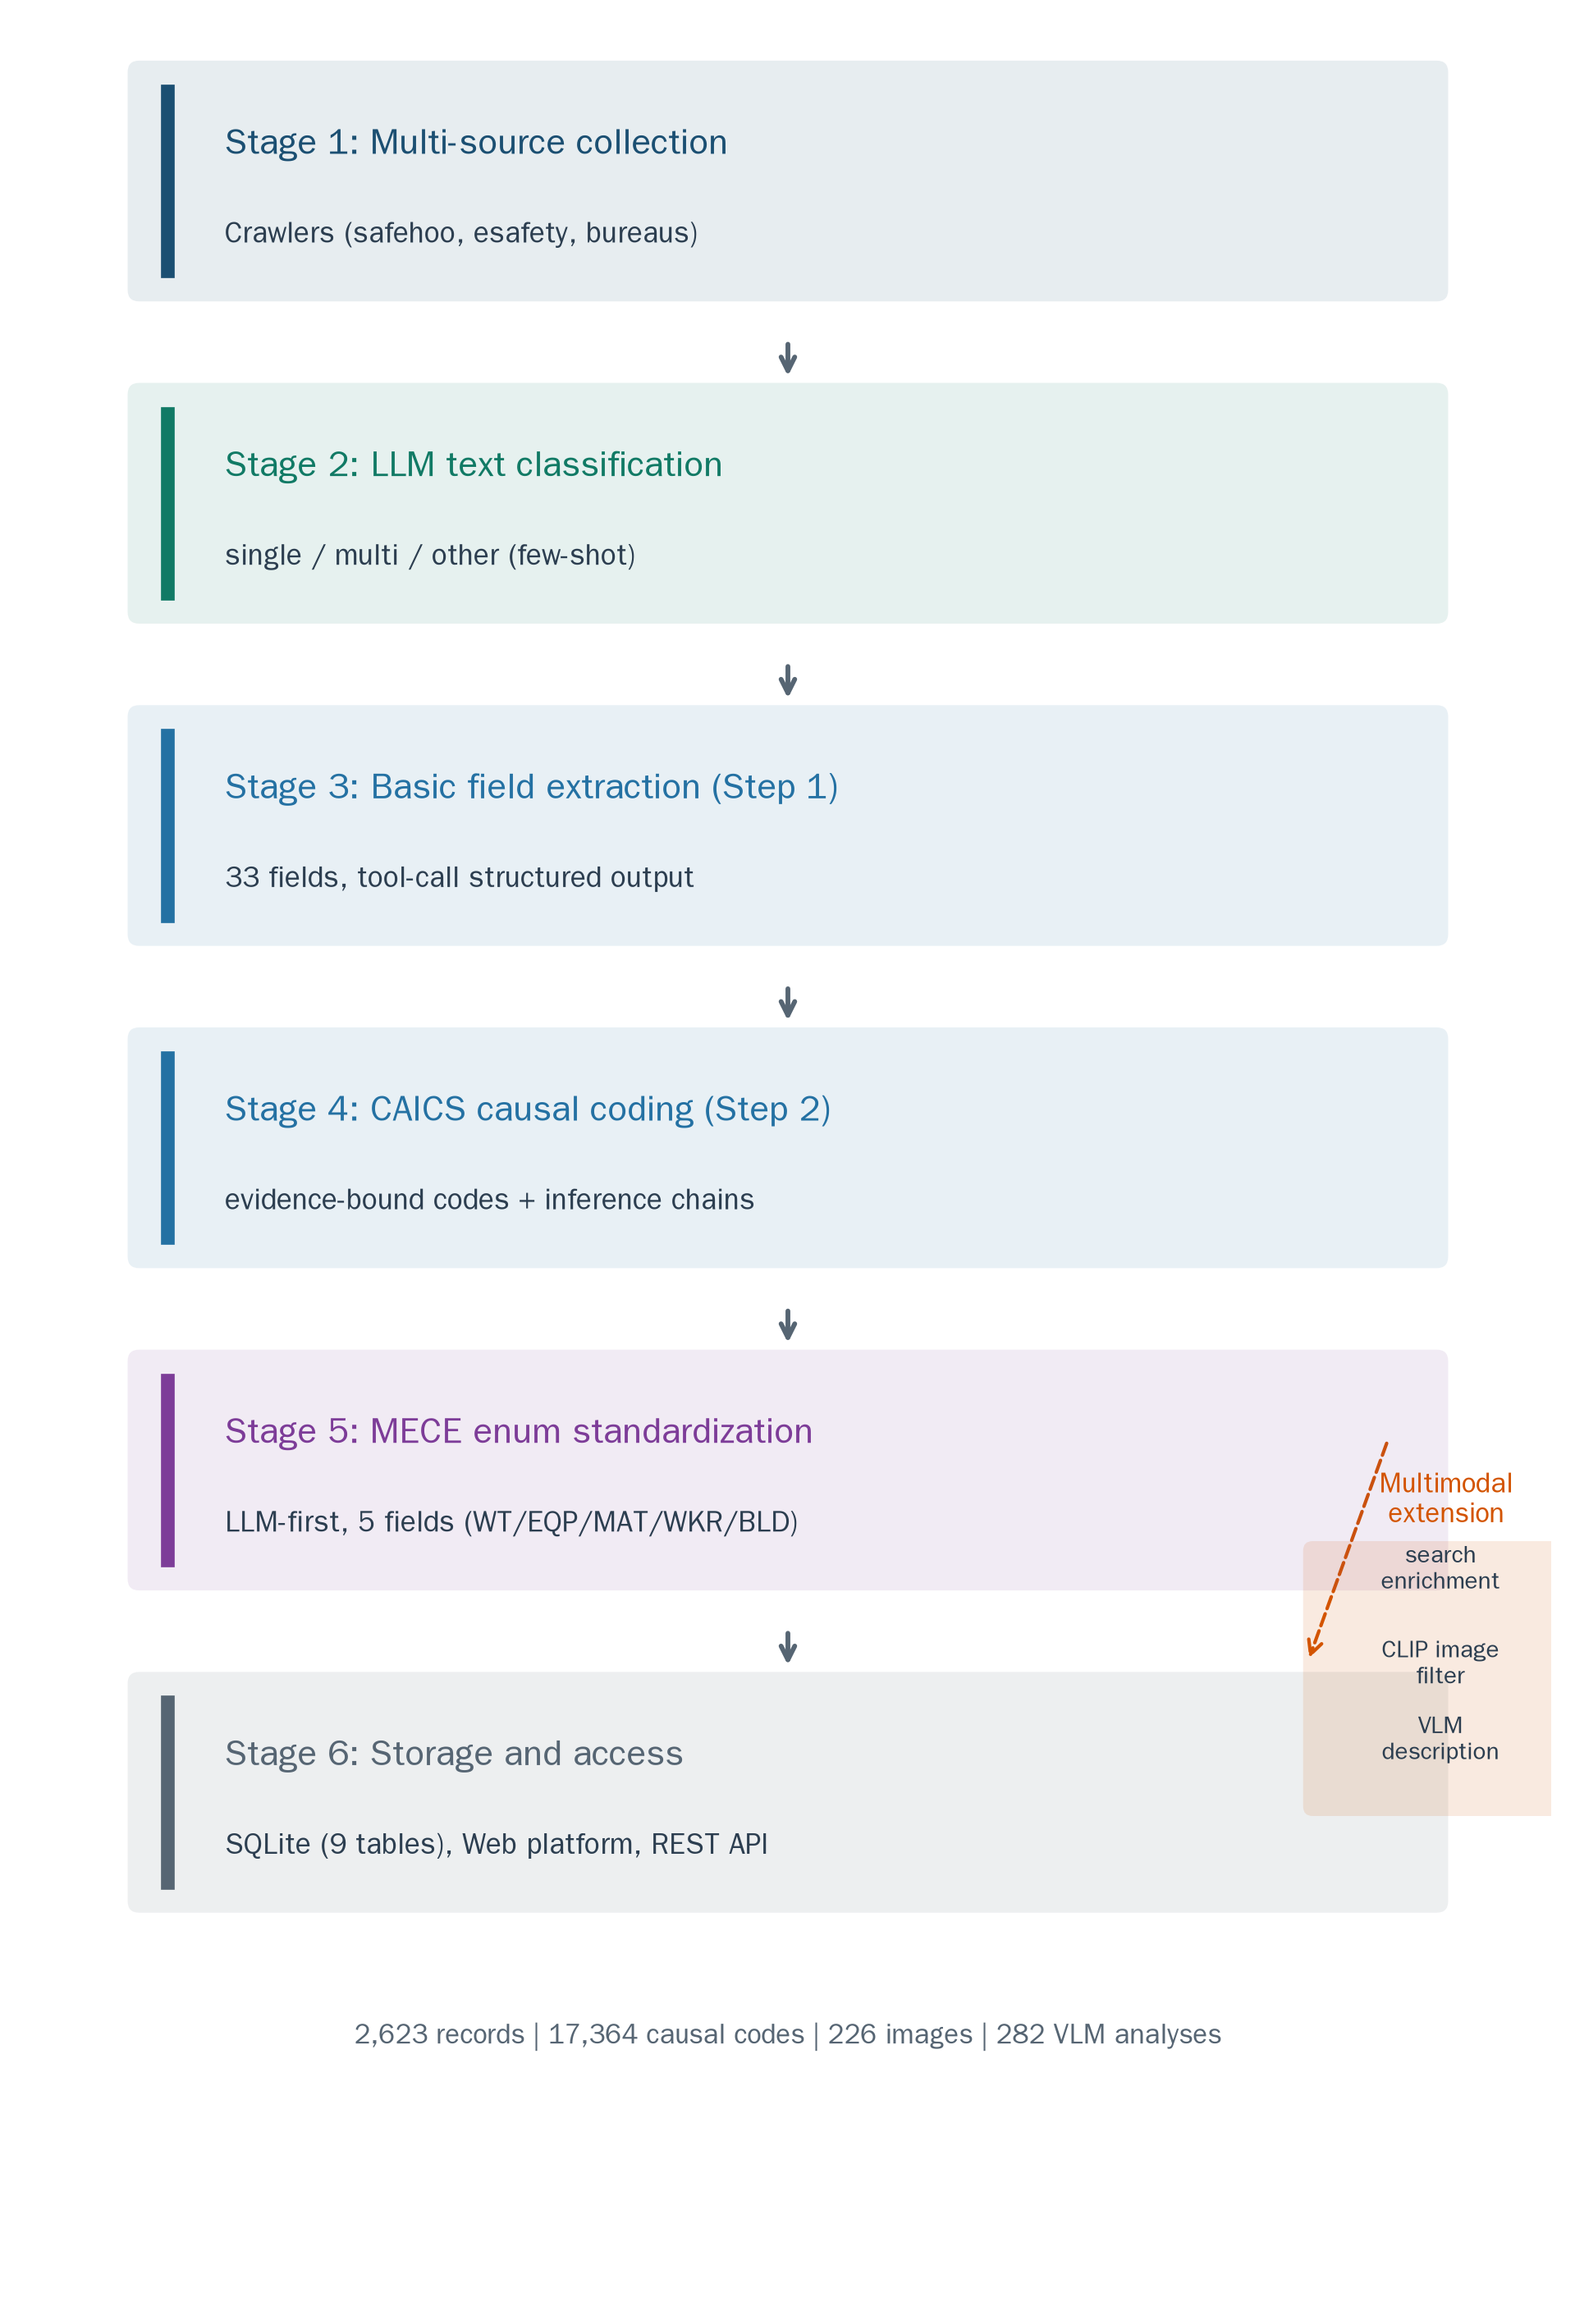
\includegraphics[width=0.85\textwidth]{figures/fig1_architecture.png}
\end{figure}
\textbf{Stage 1: Multi-source collection.} A crawler ingests accident reports from public safety information portals (safehoo.com, esafety.cn) and local emergency-management bureaus. Raw HTML is parsed into structured fields (title, publication date, body text, source URL) and stored as candidate records. The corpus assembled for this paper spans 1978 to 2026 and covers all 31 provincial-level regions of mainland China.

\textbf{Stage 2: LLM-based text classification.} Candidate records are heterogeneous: many pages contain multiple accidents, safety regulations, textbook excerpts, or advertisements. A lightweight LLM classifier assigns each record one of three text types: \textit{single} (one accident narrative), \textit{multi} (several accidents, split before further processing), or \textit{other} (non-accident content, archived without extraction). The classifier uses few-shot prompting with five annotated examples covering the three classes. This stage removed 895 textbook-derived records and all advertisement and navigation pages, yielding 2,623 single-accident records.

\textbf{Stage 3: Basic field extraction (Step 1).} For each accepted record, an LLM extracts the 33-field basic information vector under a strict JSON tool schema. Structured-output enforcement (tool-calling with a typed schema rather than free-form JSON parsing) eliminates the format-drift failures that plague unstructured output pipelines: in our runs, schema-conformant output was obtained for 100\% of records. The extractor also produces a normalized title summary, which later serves as the primary query for search enrichment (Section 3.4).

\textbf{Stage 4: CAICS causal coding (Step 2).} The coded output follows the two-step judgment procedure that emerged from our diagnostic experiments (Section 4.4). The encoder first identifies the accident's causal structure from the narrative, then matches each identified cause pattern to CAICS codes, quoting verbatim evidence and recording the inference chain for every code. Figure 2 illustrates the five-layer causal structure with an example chain extracted from a real record.

\textbf{Figure 2.** CAICS five-layer causal structure with an example evidence chain.}
\begin{figure}[H]
\centering
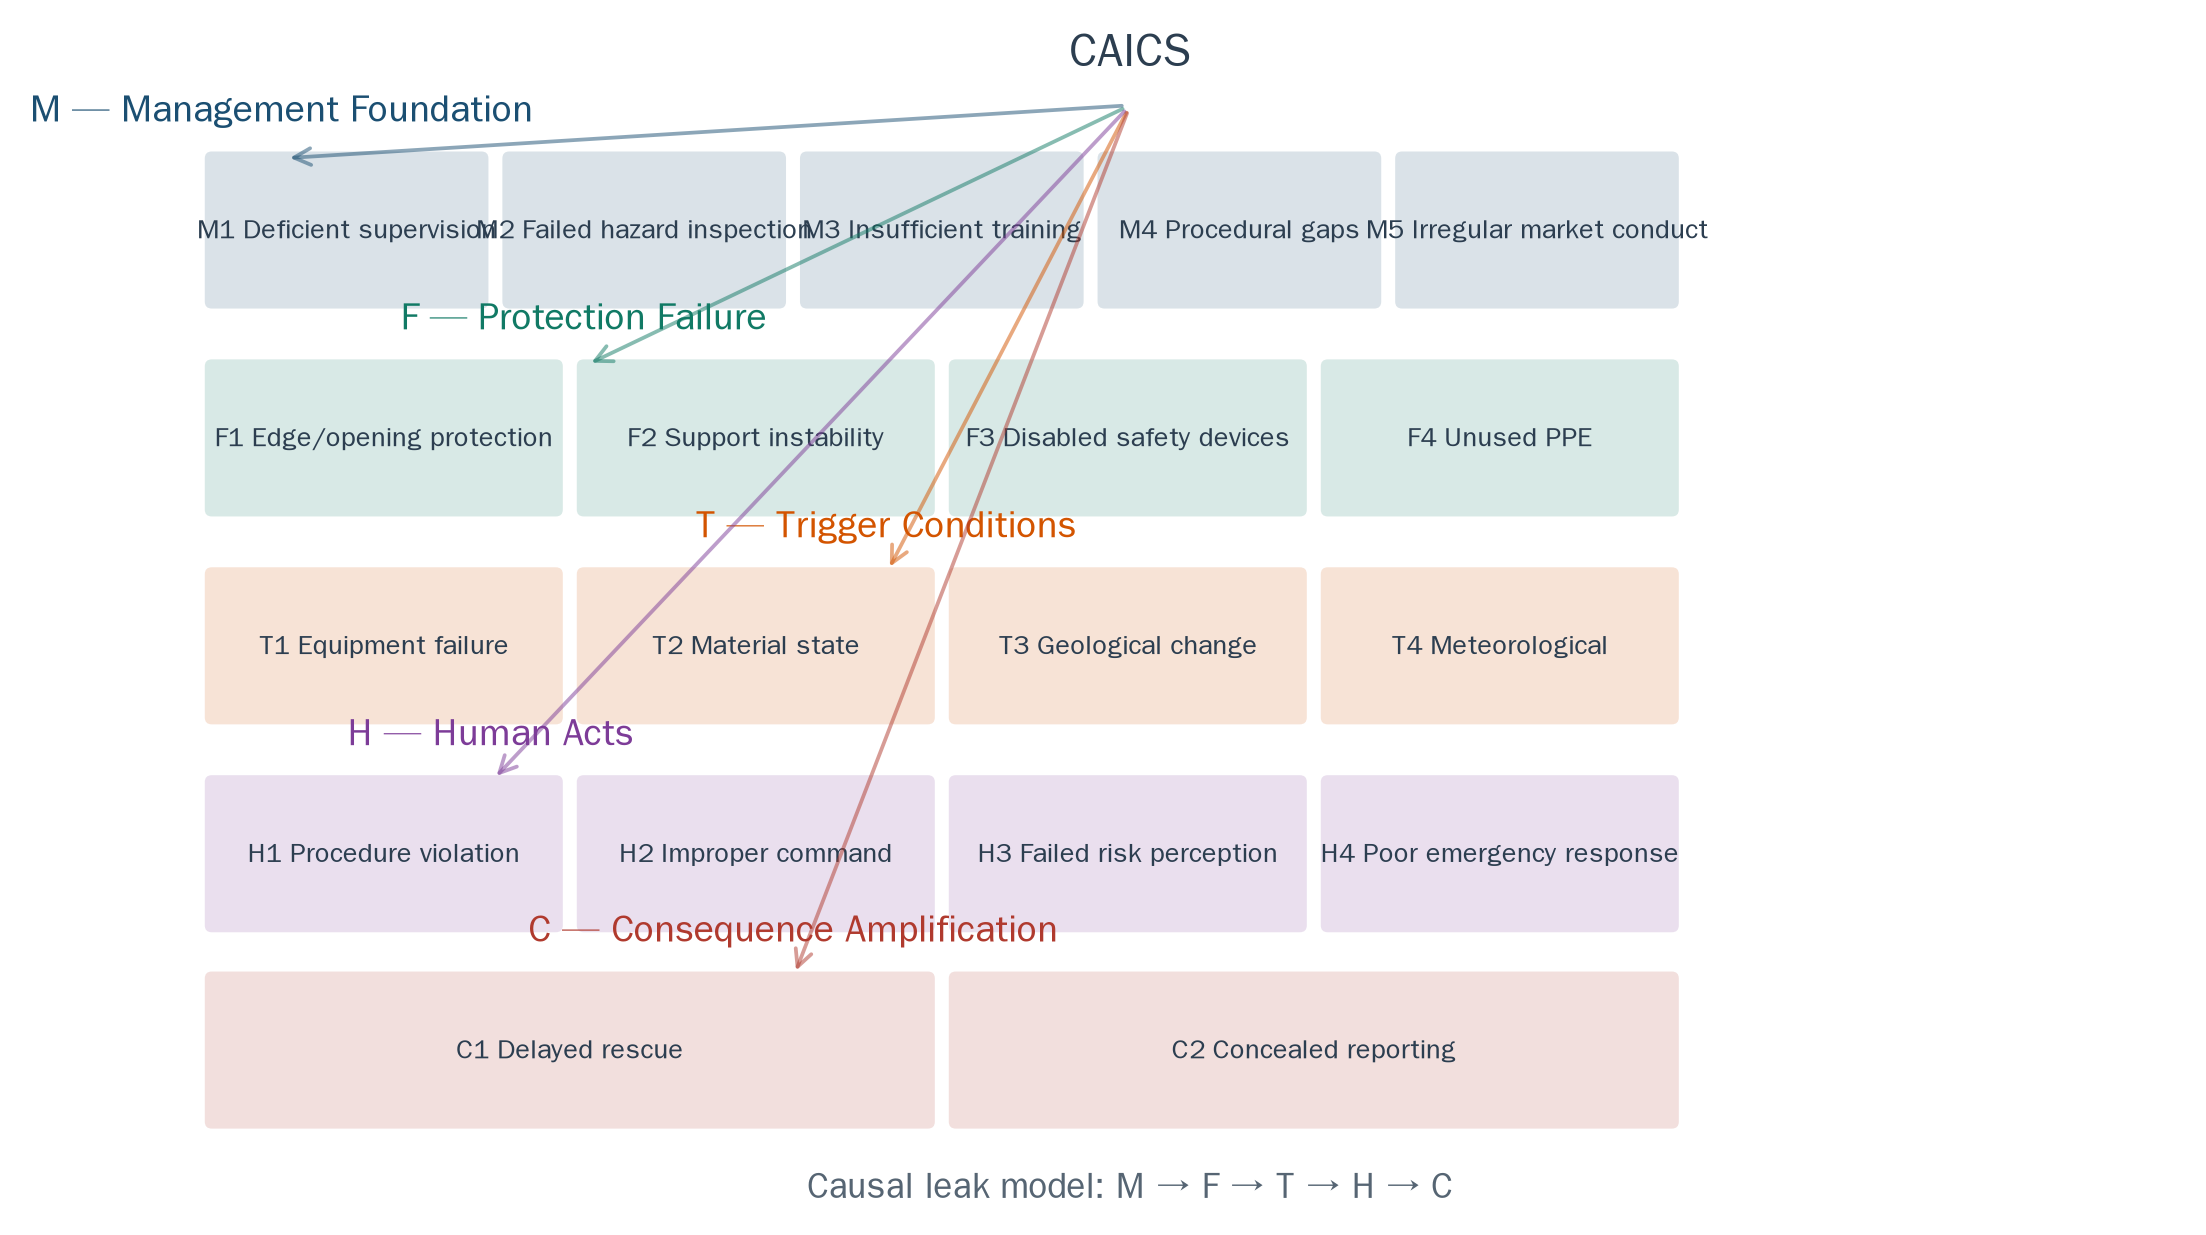
\includegraphics[width=0.85\textwidth]{figures/fig2_caics_tree.png}
\end{figure}
\textbf{Stage 5: LLM-first MECE enum standardization.} Five basic fields (work task, equipment involved, material involved, worker type, building structure) are free-text in the source narratives. We standardize them through an LLM-first enumeration procedure that operationalizes the MECE principle: the LLM reviews the complete value distribution of a field across the corpus, designs a category framework satisfying mutual exclusivity and collective exhaustiveness, and then maps every observed value onto the framework. The procedure runs in two phases with different model configurations: framework design uses a high-capacity configuration, and full-corpus mapping uses a lightweight configuration for cost efficiency. This design inverts the conventional rule-first approach, in which an analyst prescribes categories before observing the data and subsequently encounters unmappable values. Table 2 reports the resulting enumerations. For the work task field, the LLM merged six original categories into four and introduced one new category (auxiliary work and on-site transport), reducing the residual "other" share from 18.9\% to 2.9\%.

\textbf{Table 2.** MECE enumerations produced by the LLM-first procedure.}
\begin{table}[htbp]
\centering
\small
\begin{tabular}{crcc}
\hline
Field & Categories & Largest category (share) & Residual "other" \\
\hline
Work task (WT) & 11 & WT02 main structure works (397, 18.0\%) & 2.9\% \\
Equipment involved (EQP) & 13 & EQP01 hoisting machinery (335, 24.4\%) & 1.9\% \\
Material involved (MAT) & 7 & MAT01 concrete and cement products (423, 28.9\%) & 11.1\% \\
Worker type (WKR) & 13 & WKR01 general laborers (928, 48.7\%) & 6.3\% \\
Building structure (BLD) & 12 & BLD01 steel structures (127, 35.4\%) & 3.6\% \\
\hline
\end{tabular}
\end{table}
\textbf{Stage 6: Storage and access.} All artifacts (records, causal codes, enumerations, images, analyses) are stored in a SQLite relational database with nine tables. The final database contains 2,623 accident records, 17,364 evidence-bound causal codes (6.6 codes per record on average), and 33 standardized fields per record. An interactive Web platform and REST API expose the database: users can filter accidents by type, severity, region, work task, and causal code, and can inspect the evidence chains behind every causal annotation. The database is released publicly upon publication (Data Availability Statement, Section 7).

\subsection{3.4 Multimodal Extension}
Beyond text, the pipeline enriches records with web-sourced materials through three modules. First, a search-enhancement module queries an aggregated search API with the extracted title and the city-and-type pair, retrieving supplementary news coverage; 1,636 records (62.4\%) were enriched with additional sources. Second, an image-collection module extracts candidate images from the retrieved pages and filters them with a zero-shot CLIP classifier (openai/clip-vit-base-patch32) that distinguishes accident-scene photographs from logos, icons, and decorations; 226 images passed the 0.5 similarity threshold. Third, a vision-language analysis module (GLM-5V-Turbo) produces a two-phase description per image: a blind observation pass over scene, damage, weather, and personnel, followed by a fusion pass that combines the observation with the record's Step 1 fields into an 80--150 character multimodal summary; 282 analyses covering 176 accidents were stored in the database. We emphasize that the multimodal modules are display-oriented extensions: image quality at the source (news-page thumbnails and compressed photographs) remains the binding constraint, and VLM output is presented as supplementary description rather than as verified annotation. This positioning is deliberate and documented in the limitations (Section 5.4).

\subsection{3.5 Database Statistics}
Table 3 summarizes the database. The severity distribution follows the Chinese classification standard for production safety accidents (general, relatively major, major, and particularly major). The twelve accident types consolidate the standard Chinese occupational-injury classification (GB 6441-86) with construction-specific granularity: collapse and earthwork collapse are separated because they dominate construction fatalities and require distinct preventive regimes, while drowning and poisoning/asphyxiation are retained as distinct types despite their lower frequency. Two temporal blocks compose the corpus: a historical block (1978--1990, 698 records, 26.6\%), digitized from a published accident compilation, and the contemporary block (2005--2026, 1,925 records, 73.4\%) collected from news portals; 1991--2004 is unrepresented. Reports also include accidents at overseas sites of Chinese contractors (22 records with foreign locations), which are retained in the database but excluded from the provincial coverage statistics. The causal-code distribution across the nineteen CAICS categories is reported in Figure 3; the top codes (M1 deficient supervision, H1 procedure violation, H3 failed risk perception) are consistent with the management-rooted causal structure expected from the leak model.

\textbf{Table 3.** Database statistics.}
\begin{table}[htbp]
\centering
\small
\begin{tabular}{cc}
\hline
Dimension & Value \\
\hline
Records & 2,623 \\
Time span & 1978-08 to 2026-06 \\
Provinces covered & 31 \\
Accident types & 12 (collapse 1,092; fall-from-height 570; hoisting 225; earthwork collapse 222; electrocution 160; struck-by 119; other 50; fire/explosion 47; mechanical 46; poisoning/asphyxiation 41; vehicle 38; drowning 7) \\
Severity & general 1,889; relatively major 672; major 53; particularly major 8 \\
Casualties & 5,894 deaths; 5,796 injuries \\
Causal codes & 17,364 (mean 6.6 per record) \\
Search-enriched records & 1,636 \\
CLIP-filtered images & 226 \\
VLM analyses & 282 across 176 accidents \\
\hline
\end{tabular}
\end{table}
\textbf{Figure 3.** Distribution of causal codes across the nineteen CAICS categories.}
\begin{figure}[H]
\centering
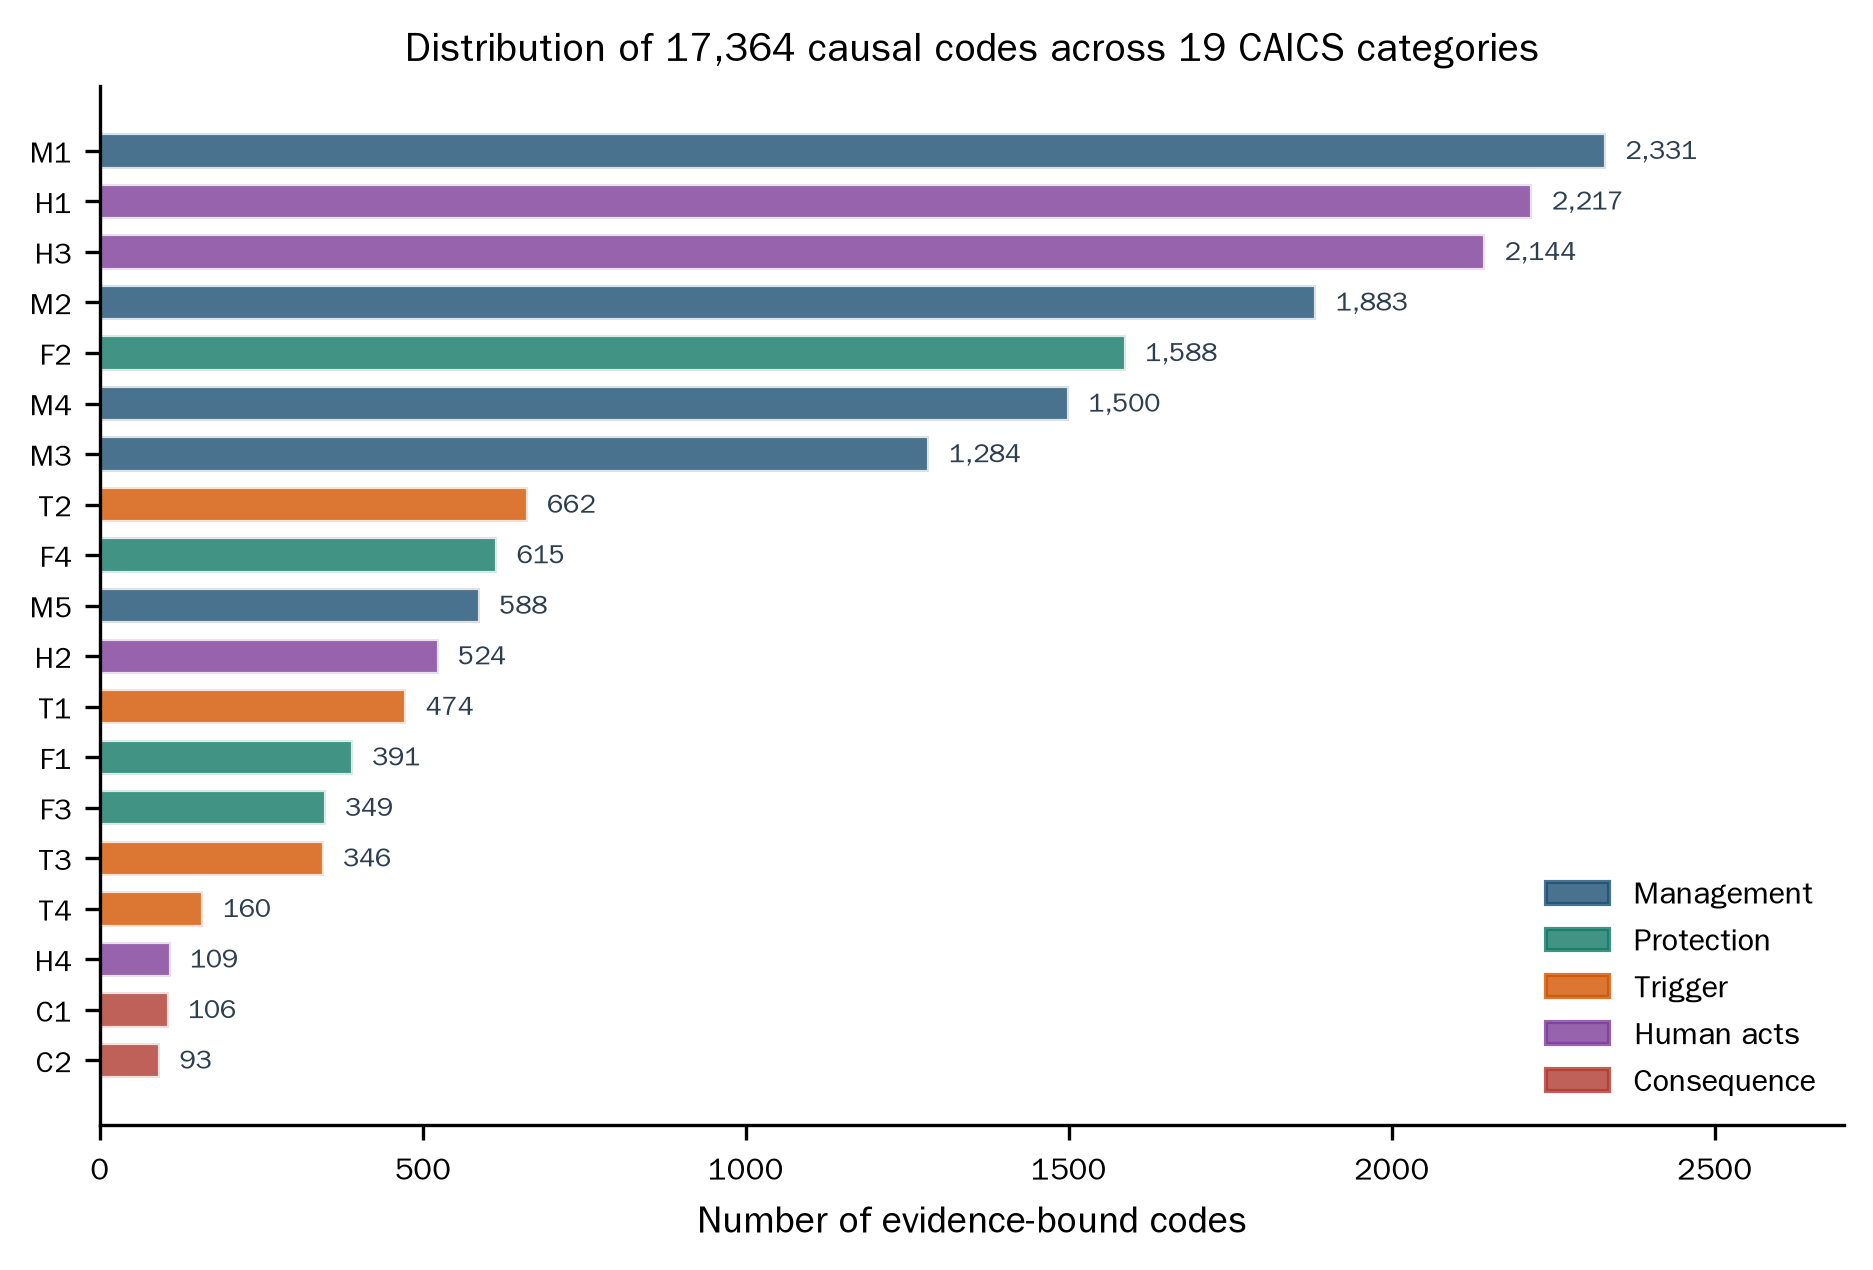
\includegraphics[width=0.85\textwidth]{figures/fig3_code_dist.png}
\end{figure}
\textbf{Figure 4.** The CAIEMS web platform: interactive browsing of the database (2,623 records).}
\begin{figure}[H]
\centering
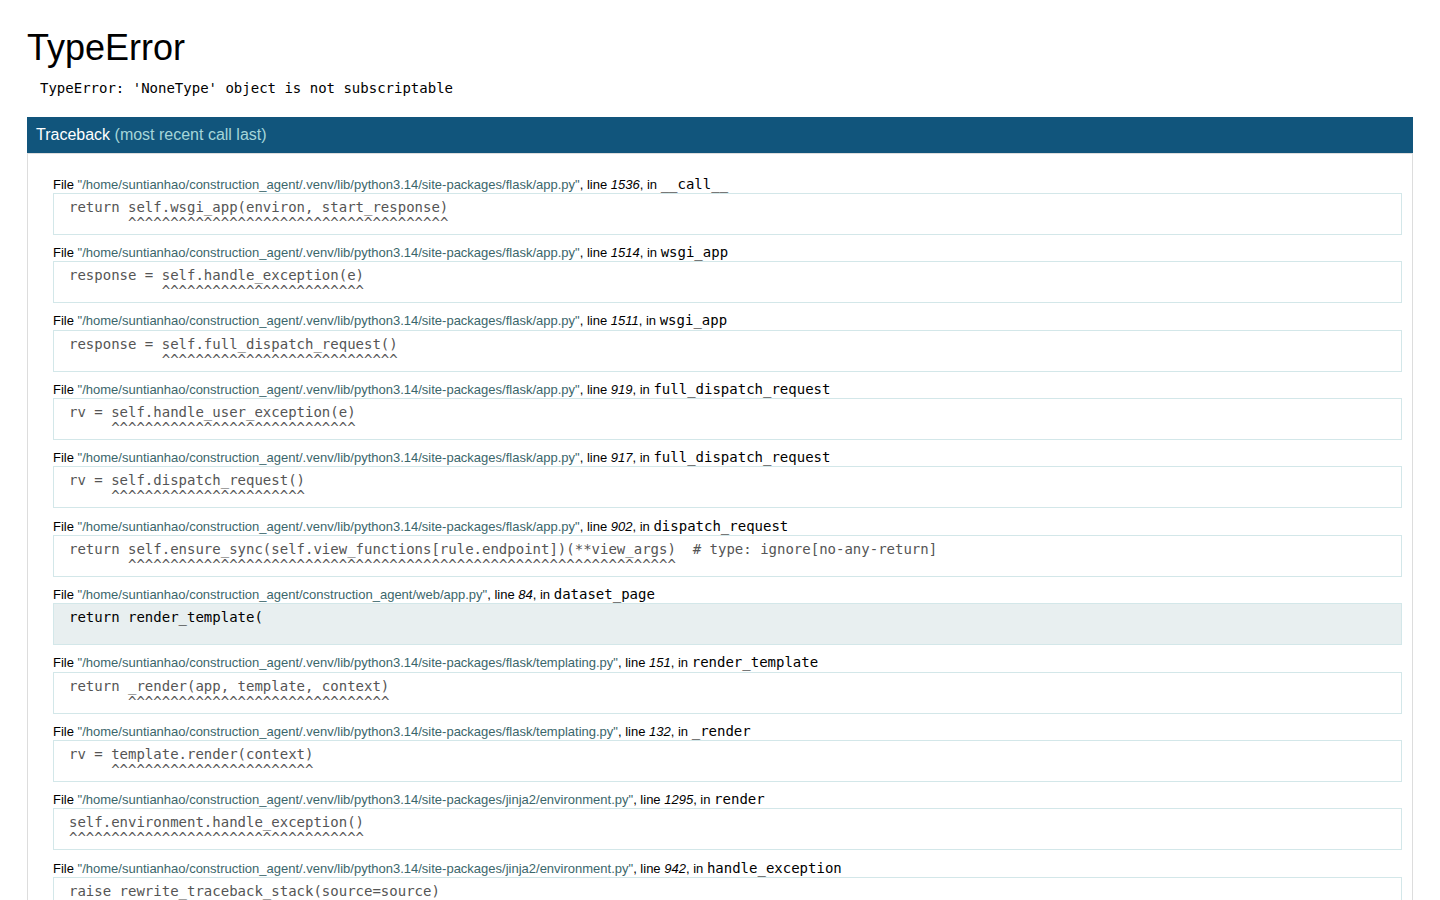
\includegraphics[width=0.85\textwidth]{figures/web_dataset.png}
\end{figure}
\section{4. Experimental Evaluation}
The evaluation addresses three questions in sequence: which backbone model should drive the pipeline (Section 4.3), how should that model be prompted for causal coding (Section 4.4), and whether the resulting annotations are trustworthy at the scale of human expert labeling (Section 4.5). Sections 4.1 and 4.2 define the datasets and metrics shared by all three experiments.

\subsection{4.1 Datasets and Sampling}
\textbf{Full corpus.} The pipeline (Section 3.3) produced 2,623 single-accident records spanning 1978 to 2026, with 33 standardized fields and 17,364 evidence-bound CAICS codes.

\textbf{Silver standard.} For controlled evaluation, we maintain a silver-standard subset of 972 records constructed through multi-source agreement: basic fields (accident type, severity, casualties, province) were adopted directly when two independent pipeline versions agreed, resolved by rule-based arbitration when they disagreed, and causal-dimension labels were formed by merging the two versions' outputs with deduplication. An empty causal dimension in the silver standard indicates that the dimension is not mentioned in the source text (an annotation decision, not a missing label). A 100-record subset of this silver standard received fully independent human validation: three construction-safety experts annotated the CAICS codes on the LabelStudio platform, with Fleiss' Kappa exceeding 0.85 on every CAICS layer (Section 4.4). Three evaluation samples are drawn from this hierarchy:

1. \textit{Model selection sample} ($n=200$). Stratified by accident type (11 classes, minimum three per class) drawn from the silver standard, used in Experiment 1. 2. \textit{Strategy comparison sample} ($n=100$). Drawn from the silver standard covering all 12 accident types and all 19 CAICS categories; the causal ground truth was built by majority vote of three construction-safety experts labeling independently on the LabelStudio platform, with Fleiss' Kappa between 0.859 and 1.000 across the five CAICS layers (verified from the recovered annotations; the ground truth carries 5.1 codes per record on average). 3. \textit{Agreement sample} ($n=289$). Two-stage stratified random sampling (accident type $\times$ severity, proportional allocation with a floor of two per cell) from the full 2,623-record population; the resulting sample distribution deviates from the population by less than 1.5\%. A safety-engineering graduate student annotated six basic features (accident type, severity, province, deaths, injuries, date) via LabelStudio. Eleven records drawn from the original 300 were excluded as multi-accident texts, yielding the final $n=289$.

Figure 5 summarizes the sample hierarchy.

\textbf{Figure 5.** Dataset hierarchy and the three evaluation samples.}
\begin{figure}[H]
\centering
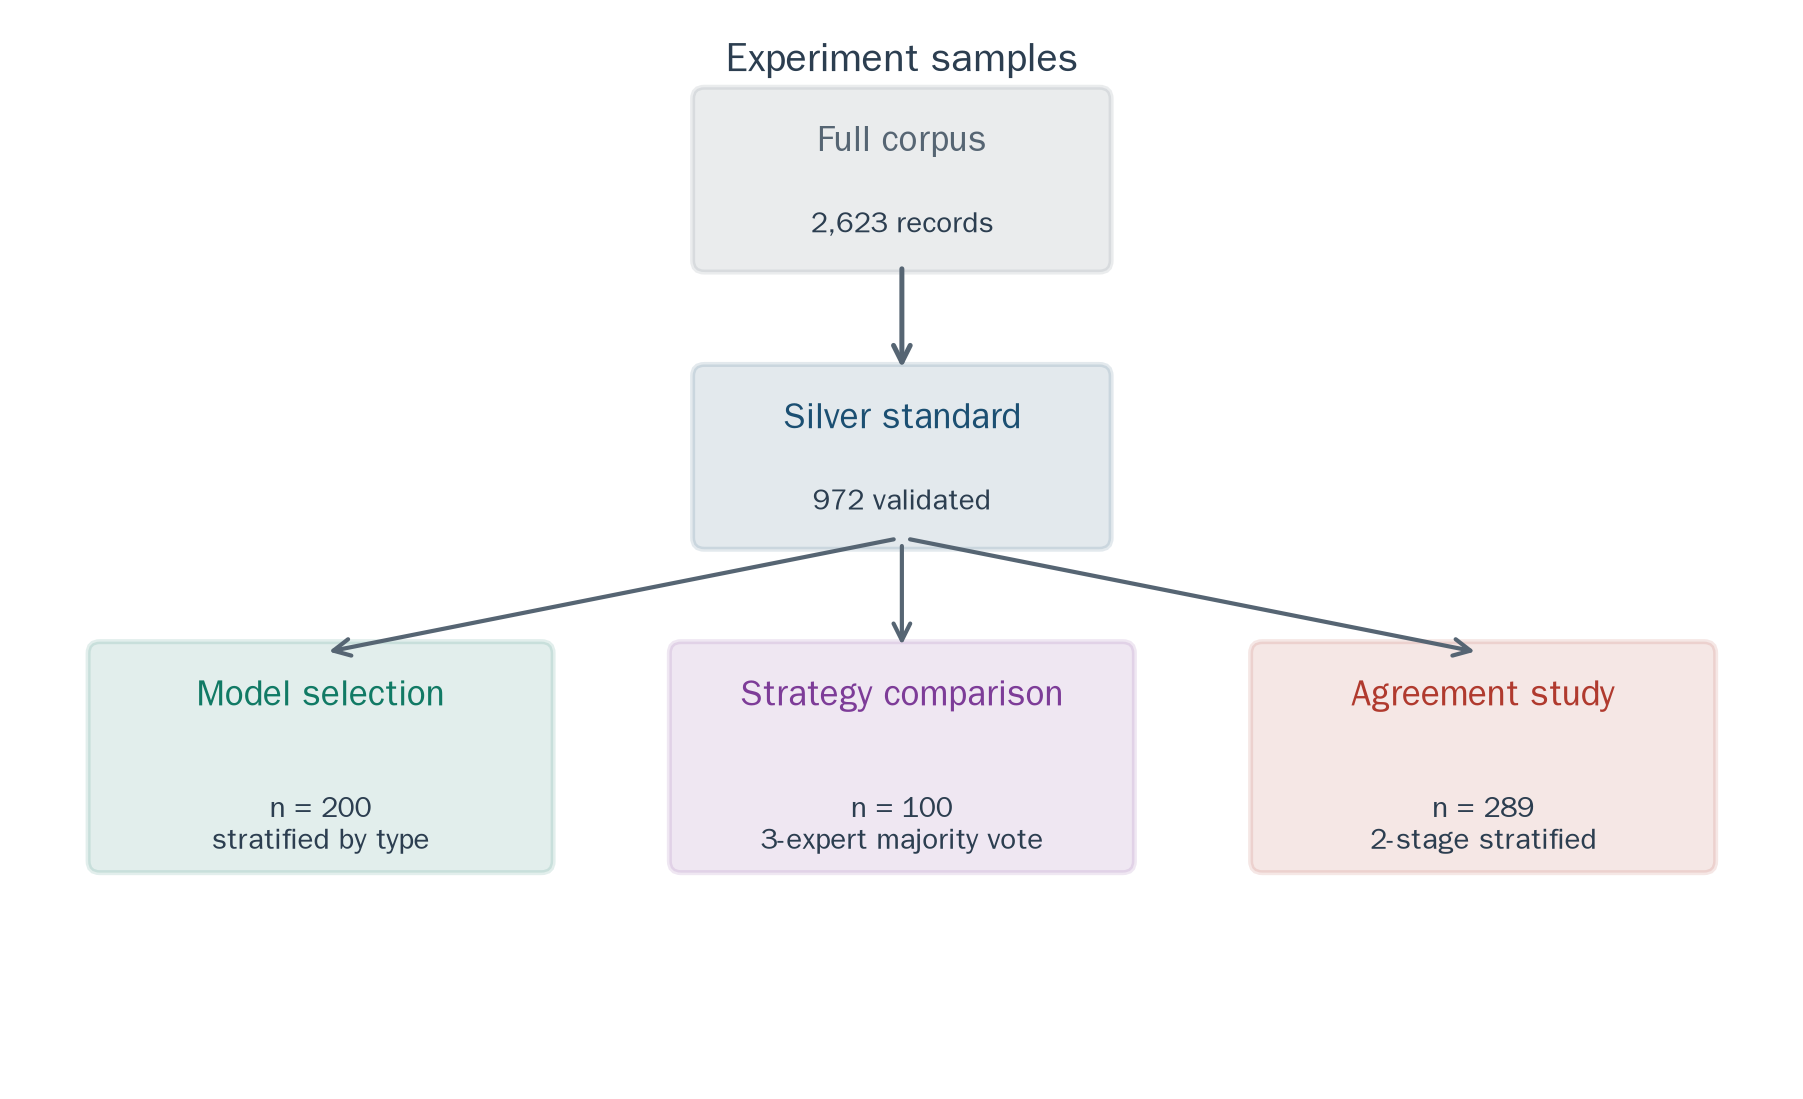
\includegraphics[width=0.85\textwidth]{figures/fig5_sampling.png}
\end{figure}
\subsection{4.2 Evaluation Metrics}
For basic field extraction we report exact-match accuracy per field, with administrative-suffix normalization for location fields (e.g., "{\cjkfont 广东}" and "{\cjkfont 广东省}" treated as equivalent). For causal coding we report precision, recall, and F1 computed per dimension (management, protection, trigger, human, consequence) by comparing each model's extracted codes against the ground-truth codes, using the dimension-level match definition of Liu et al. [8]. For human-AI agreement we use Cohen's kappa with 95\% confidence intervals for categorical fields, the intraclass correlation coefficient ICC(2,1) for count fields, and year-month match rate for dates.

\subsection{4.3 Experiment 1: Backbone Model Selection}
Four candidate backbone models were evaluated on the model selection sample: DeepSeek V4, Qwen 3.7, GLM 5.2, and Kimi K2.6. All models received an identical system prompt specifying the 33-field JSON schema and the same three few-shot examples; temperature was set to 0.0 for deterministic output, with two documented exceptions: Kimi K2.6 enforces temperature 1.0 by API specification, and GLM 5.2, a reasoning-oriented model, required a 16,384-token output budget to accommodate its chain-of-thought traces. No search enhancement was applied, isolating each model's intrinsic extraction capability. DeepSeek V4 was accessed through the provider's official API with automatic tier routing enabled; the recorded request identifiers span the DeepSeek V4 tier family, and the experiments reflect the provider's routing behavior as operated. Reproducible runs should pin the tier explicitly.

Table 4 reports per-field accuracy. The three strongest models are statistically indistinguishable on basic fields (91.2--91.5\% overall), with uniformly high accuracy on severity (90.5--98.0\%), death toll (96.0--97.0\%), and provincial location (96.0--98.5\%). City extraction is the hardest field (81.5--88.0\%): Chinese reports frequently name county-level cities, while the silver standard records the parent prefecture-level city, so a geographically correct output such as "{\cjkfont 华蓥市}" is penalized against ground truth "{\cjkfont 广安市}". Kimi K2.6 lags far behind (63.9\%) because its enforced temperature of 1.0 produced malformed JSON in 12.5\% of cases and unstable outputs across fields.

\textbf{Table 4.** Basic field extraction accuracy (\%), Experiment 1.}
\begin{table}[htbp]
\centering
\small
\begin{tabular}{ccccc}
\hline
Field & DeepSeek V4 & Qwen 3.7 & GLM 5.2 & Kimi K2.6 \\
\hline
Accident type & 86.0 & 85.0 & 84.5 & 61.5 \\
Severity & 98.0 & 90.5 & 97.5 & 69.5 \\
Deaths & 96.0 & 96.0 & 97.0 & 68.5 \\
Injuries & 90.0 & 91.0 & 91.0 & 58.5 \\
Province & 96.0 & 98.5 & 96.0 & 67.0 \\
City & 81.5 & 88.0 & 83.0 & 58.5 \\
Overall & 91.2 & 91.5 & 91.5 & 63.9 \\
\hline
\end{tabular}
\end{table}
Causal coding reveals a sharper contrast, shown in Table 5. DeepSeek V4 achieves the highest average precision (89.5\%) at the cost of the lowest recall among the capable models (52.7\%). Qwen 3.7 mirrors this trade-off in the opposite direction (78.0\% precision, 80.5\% recall). Inspection of the outputs shows that this divergence reflects extraction philosophy rather than raw capability: DeepSeek V4 emits a causal code only when the source text carries explicit linguistic evidence, while Qwen 3.7 infers causes from contextual cues even without explicit causal language. For database construction, precision is the binding constraint: every hallucinated cause injects noise into all downstream analyses, whereas a missed cause leaves the record merely incomplete. DeepSeek V4's conservative posture --- extraction faithfulness --- is the appropriate design property for this system. This position complements Liu et al. [8], who prioritized recall in exploratory aviation analysis and accepted lower precision.

\textbf{Table 5.** Causal coding precision / recall / F1 (\%) by dimension, Experiment 1.}
\begin{table}[htbp]
\centering
\small
\begin{tabular}{ccccc}
\hline
Dimension & DeepSeek V4 & Qwen 3.7 & GLM 5.2 & Kimi K2.6 \\
\hline
Management & 89.9 / 54.9 / 68.1 & 67.5 / 95.6 / 79.1 & 92.3 / 63.7 / 75.4 & 97.6 / 36.3 / 52.9 \\
Protection & 91.9 / 41.9 / 57.6 & 88.8 / 64.0 / 74.4 & 87.6 / 67.6 / 76.3 & 96.4 / 39.0 / 55.5 \\
Trigger & 81.0 / 69.4 / 74.7 & 72.4 / 85.7 / 78.5 & 73.9 / 69.4 / 71.6 & 81.5 / 44.9 / 57.9 \\
Human & 95.0 / 44.7 / 60.8 & 83.3 / 76.5 / 79.8 & 83.9 / 61.2 / 70.7 & 88.2 / 35.3 / 50.4 \\
Average & 89.5 / 52.7 / 65.3 & 78.0 / 80.5 / 78.0 & 84.4 / 65.5 / 73.5 & 90.9 / 38.9 / 54.2 \\
\hline
\end{tabular}
\end{table}
Three operational factors complete the selection picture. Cost over the 200-record sample: USD 0.13 (DeepSeek V4), 0.43 (Qwen 3.7), 2.91 (GLM 5.2), 2.84 (Kimi K2.6); extrapolated to the full 972-record silver standard, DeepSeek V4 projects to USD 0.63 against USD 14.14 for GLM 5.2, a 22-fold gap. Latency per record: 9.8 s (DeepSeek V4), 8.6 s (Qwen 3.7), 27.0 s (GLM 5.2), 74.9 s (Kimi K2.6). Output validity: DeepSeek V4 and Qwen 3.7 produced schema-conformant output for all 200 records, GLM 5.2 for 197, Kimi K2.6 for 140. DeepSeek V4 occupies the favorable corner of the performance-cost frontier, and we selected it as the backbone of CAIEMS. Its Anthropic-compatible and OpenAI-compatible API interfaces further simplify deployment in the Chinese computing environment, where direct access to foreign endpoints is unreliable.

\subsection{4.4 Experiment 2: Prompt Strategy Comparison and the Lexical Gatekeeping Effect}
Six prompting strategies were compared on the strategy comparison sample ($n=100$, three-expert majority-vote ground truth) using DeepSeek V4 (temperature 0.0), following the strategy taxonomy of Liu et al. [8]: S0 Basic Zero-Shot, S1 Basic Few-Shot (three expert-annotated examples), S2 Auto-CoT, S3 Plan-and-Solve, S4 CAICS-CoT (our domain-knowledge CoT design), and S5 CAICS-CoT+ (our serial per-layer architecture with five independent API calls and inter-layer summaries). Appendix A reproduces all six prompts.

\textbf{Table 6.** Performance of six prompting strategies (majority-vote ground truth, n = 100).}
\begin{table}[htbp]
\centering
\small
\begin{tabular}{cccccccc}
\hline
Strategy & Avg. F1 [95\% CI] & Avg. Recall & Avg. Precision & Type acc. & Severity acc. & Valid-output rate & Time (s) \\
\hline
S0 Zero-Shot & 0.600 [0.520, 0.644] & 0.515 & 0.808 & 0.630 & 0.960 & 96\% & 1,382 \\
S1 Few-Shot & 0.669 [0.615, 0.722] & 0.634 & 0.753 & 0.840 & 0.970 & 100\% & 1,302 \\
S2 Auto-CoT & 0.634 [0.564, 0.691] & 0.564 & 0.772 & 0.860 & 0.980 & 85\% & 2,401 \\
S3 Plan-and-Solve & 0.598 [0.529, 0.652] & 0.540 & 0.741 & 0.850 & 0.990 & 92\% & 1,735 \\
S4 CAICS-CoT & 0.656 [0.603, 0.695] & 0.872 & 0.565 & 0.830 & 0.990 & 99\% & 1,843 \\
S5 CAICS-CoT+ & 0.665 [0.606, 0.719] & 0.750 & 0.618 & 0.830 & 0.980 & 100\% & 5,430 \\
\hline
\end{tabular}
\end{table}
\textit{\textit{Notes.} Ground truth is the majority vote of three independent expert annotators (Fleiss' Kappa > 0.85 on every CAICS layer, Section 4.1). Confidence intervals are percentile bootstrap (1,000 resamples). S2's type/severity accuracy is unevaluable because its prompt did not request those fields. S2's coding metrics were computed after a post-processing step that recovered 96/100 outputs exhibiting hierarchical-format drift (`{M:[...], F:[...]}` instead of `{codes:[...]}`); no other strategy received post-processing, so S2's F1 is an upper-bound estimate of a post-processed pipeline rather than a strictly comparable raw-output score. All strategies ran once at temperature 0.0.}\\
Three findings structure this section. First, Few-Shot outperforms all strategies, including both domain-knowledge CoT designs (0.669 vs. 0.656), which reverses the ranking established by Liu et al. [8] on GPT-4o, where domain CoT dominated Few-Shot. Second, our CoT design S4, while not the top strategy on F1, delivers the highest recall by a wide margin (0.872), and its v1-to-v2 iteration produced the diagnostic evidence for the Lexical Gatekeeping Effect. Third, the serial architecture S5 matches S4 on F1 (0.665 vs. 0.656, overlapping CIs) but requires six times the API calls and 2.9 times the wall-clock time, contradicting its design rationale of improving per-layer quality through isolation.

S1's examples perform joint format-content calibration: they demonstrate not only the output schema but the expected code density (five to seven codes per record), code combination patterns (management codes nearly always present, human codes frequently co-occurring), and inference depth. The model internalizes these norms through in-context learning rather than through explicit instructions. Notably, S1's average code density closely matched the ground truth (5.0 vs. 5.1), while S0 under-coded (3.6) and S4 over-coded (6.5); few-shot examples act as an implicit output-length calibrator that no textual instruction reproduced.

The reversal relative to Liu et al. [8] admits two confounded readings, because the comparison differs in model (GPT-4o vs. DeepSeek V4) and in task (aviation HFACS vs. construction CAICS) simultaneously. The ranking difference could be model-dependent, task-dependent, or both. We report it as a robust empirical contrast rather than a clean causal attribution: whichever factor dominates, the practical consequence is the same --- the optimal prompting strategy for a new domain-model pair cannot be assumed from a single published ranking. A plausible capability-profile explanation exists (DeepSeek V4's code-heavy pretraining favors in-context pattern matching; GPT-4o's instruction tuning favors executing multi-step reasoning directives), but the decisive within-study test --- the same CAICS task run across multiple models --- is future work, and the model-dependence hypothesis should be read as exactly that.

The initial version of S4 (v1) embedded domain knowledge as conditional checks: each code was presented with an interrogative gate, for example "M1 deficient supervision: does the text mention 'no supervision' or 'supervision failure'?" accompanied by an instruction not to fabricate codes. The outcome was catastrophic: F1 = 0.503, recall = 0.423, 21\% of records received no codes at all, and M1 --- the most frequent ground-truth code, present in 85 of 100 records --- reached a recall of only 0.141. Most accident narratives never use the exact keyword phrases; they say "{\cjkfont 安全管理不到位}" (safety management inadequate) or "{\cjkfont 未及时发现制止}" (failure to detect and stop in time). Under the conditional-check phrasing, the model treated the listed keywords as mandatory gates rather than illustrative cues, and was effectively blind to every paraphrase.

We name this failure mode the \textbf{Lexical Gatekeeping Effect}: in conditional-check CoT prompts, an LLM converts illustrative keyword lists into necessary conditions for code emission, and paraphrased evidence that fails the literal gate is discarded, producing systematic recall collapse concentrated on the highest-frequency implicit categories.

The remedy replaces the gate with a two-step judgment: (1) explicit matching --- does the text directly support this code, with any paraphrase? (2) authorized inference --- given the accident's nature and construction-safety knowledge, is this cause necessarily present even without explicit phrasing? The conservative instruction was also replaced by a coverage preference appropriate to safety analysis, where missing a cause costs more than adding one. The combined v1$\rightarrow$v2 effects were large: F1 rose from 0.503 to 0.656, recall from 0.423 to 0.872, M1 recall from 0.141 to 0.988, and empty outputs fell from 21\% to 0. Figure 6 visualizes the recovery. Because the v1$\rightarrow$v2 transition changed two prompt properties at once (phrasing and output policy), we isolate their separate contributions with a controlled ablation below.

\textbf{Figure 6.** The Lexical Gatekeeping Effect: (a) v1$\rightarrow$v2 recovery on the strategy sample; (b) the 2$\times$2 ablation decomposing the phrasing and output-policy contributions to F1 and M1 recall.}
\begin{figure}[H]
\centering
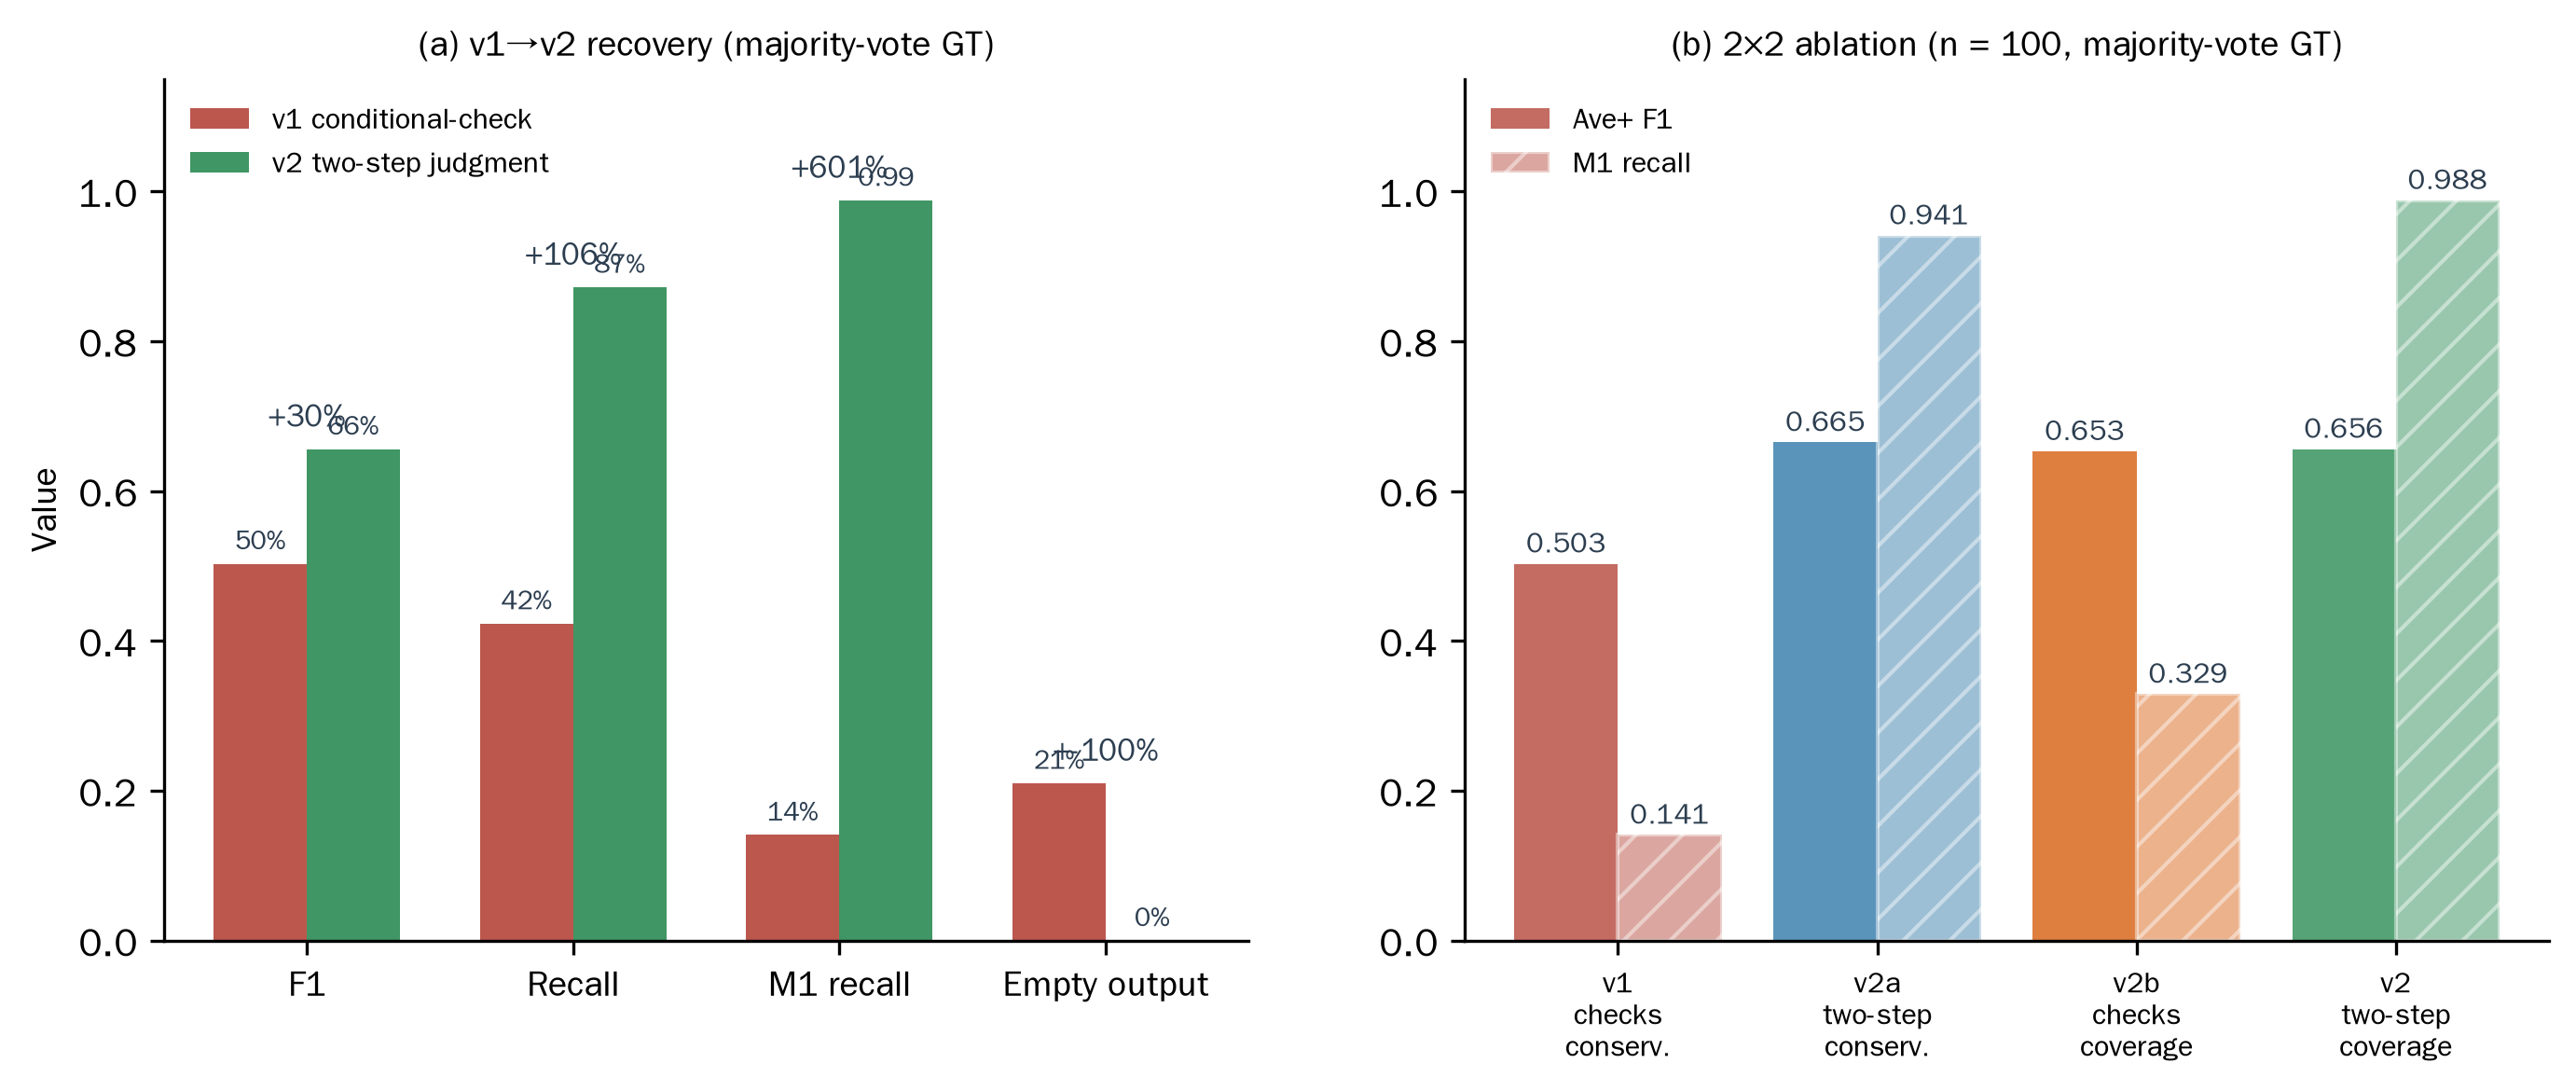
\includegraphics[width=0.85\textwidth]{figures/fig6_gatekeeping.png}
\end{figure}
The mechanism behind the effect is instructive. Interrogative phrasing ("does the text mention X?") activates the model's literal pattern-matching mode: attention concentrates on fragments containing the exact keywords, and paraphrases receive low weight. Declarative cue phrasing ("cues include a, b, c; even without these words, infer from the accident's nature") activates the reasoning mode, in which keywords define an open semantic family and the model judges membership autonomously. This asymmetry generalizes beyond construction: in any domain requiring recall-over-precision annotation (safety analysis, medical screening), CoT prompts should phrase conditions as clue guidance rather than condition checks; condition-check phrasing suits zero-false-positive settings such as legal citation.

\textbf{Controlled ablation.} To decompose the recovery into the contribution of phrasing and the contribution of the output-policy instruction, we ran a 2$\times$2 ablation on the strategy sample itself: v1 (conditional checks + conservative instruction), v2a (two-step judgment + conservative instruction), v2b (conditional checks + coverage preference), and v2 (two-step judgment + coverage preference, the production configuration). All four cells share the same 100 records, the same majority-vote ground truth, the same model and temperature (0.0). Table 7 reports the results. On the flagship implicit category M1, the decomposition is decisive: holding the conservative instruction constant, the phrasing change alone (v1 $\rightarrow$ v2a) raises M1 recall from 0.141 to 0.941 --- 0.80 of the total 0.847 recovery --- while holding phrasing constant, the policy change alone (v1 $\rightarrow$ v2b) raises it only to 0.329. At the aggregate level the two manipulations contribute comparably (F1 +0.161 vs. +0.150, recall +0.254 vs. +0.218), but their targets differ: the phrasing change unlocks the paraphrastic implicit categories that the literal gate suppresses, whereas the coverage preference lifts emission across the board. The alternative explanation that the v1 collapse merely reflected the conservative instruction --- the model suppressing all borderline codes under "do not fabricate" --- is therefore ruled out: the gatekeeping behavior is a property of the interrogative phrasing, concentrated on implicit categories whose ground-truth support is paraphrastic rather than literal.

\textbf{Table 7.** The 2$\times$2 ablation of the Lexical Gatekeeping Effect (n = 100, majority-vote ground truth, DeepSeek V4, temperature 0.0).}
\begin{table}[htbp]
\centering
\small
\begin{tabular}{cccccccccc}
\hline
Cell & Phrasing & Output policy & F1 & Recall & Precision & Empty output & M1 recall & M3 recall & H3 recall \\
\hline
v1 & Conditional checks & Conservative & 0.503 & 0.423 & 0.856 & 21\% & 0.141 & 0.250 & 0.111 \\
v2a & Two-step judgment & Conservative & 0.665 & 0.677 & 0.709 & 2\% & 0.941 & 0.667 & 0.511 \\
v2b & Conditional checks & Coverage preference & 0.653 & 0.641 & 0.724 & 5\% & 0.329 & 0.444 & 0.533 \\
v2 & Two-step judgment & Coverage preference & 0.656 & 0.872 & 0.565 & 0\% & 0.988 & 0.972 & 1.000 \\
 & $\Delta$(phrasing) = v2a − v1 &  & +0.161 & +0.254 & −0.147 & −19 pp & +0.800 & +0.417 & +0.400 \\
 & $\Delta$(policy) = v2b − v1 &  & +0.150 & +0.218 & −0.132 & −16 pp & +0.188 & +0.194 & +0.422 \\
\hline
\end{tabular}
\end{table}
The ablation also replicates the failure itself: v1's M1 recall of 0.141 reproduces the 0.143 observed in the original development run, and v1's F1 of 0.503 sits below the Zero-Shot baseline (0.600), confirming that a poorly designed domain-CoT prompt actively harms extraction.

Liu et al. [8] implicitly avoided the effect: their HFACS-CoT employed guiding rather than checking formulations, but this design convention was never stated, let alone causally verified. Our ablation provides that evidence and, to our knowledge, the first controlled decomposition of this failure mode.

S5 decomposed the five-layer analysis into five independent API calls, each performed by a layer specialist, with the prior layer's results injected as a summary. The theoretical expectation, following the design of HFACS-CoT+ [8], was that per-layer isolation prevents cross-layer attention dilution and improves per-layer quality. The result rejects the expectation: S5 attains F1 = 0.665, statistically indistinguishable from S4 (0.656, overlapping bootstrap CIs), at six times the API calls (5,430 s vs. 1,843 s for 100 records). Isolation buys nothing here; it merely redistributes the same reasoning across five truncated contexts.

The diagnosis is architectural. Each layer specialist receives a lossy summary of upstream findings ("M layer = M1, M2; F layer = F2; T layer = T2") without the reasoning that produced them. More fundamentally, CAICS causal chains are bidirectional: a trigger event (T) exposes a protection failure (F), which traces back to a management deficiency (M). A single integrated call can traverse these links freely within one reasoning context; the serial architecture truncates the chain at every layer boundary, and the truncated contexts evidently suffice to recover most of the coding quality at substantially higher cost. Liu et al. [8] found serial decomposition mildly beneficial on GPT-4o for HFACS aviation codes, whose inter-code dependencies are comparatively sparse and well-mapped. Our results suggest that for tightly coupled frameworks such as CAICS, integrated single-call reasoning with an enlarged reasoning budget is the cost-efficient design, and serial decomposition adds no measurable quality.

The production encoder (Section 3.3, Stage 4) adopts the S4 two-step judgment design rather than the empirically superior S1. The choice is deliberate: S4's recall advantage (0.872 vs. 0.634) and its evidence-bound output format serve the auditability requirement of the database. The F1 gap to S1 (0.013, within overlapping confidence intervals) is accepted as the cost of the coverage preference, consistent with the safety-domain priority established in Section 4.3.

\subsection{4.5 Experiment 3: Human-AI Agreement Validation}
The final experiment asks whether the LLM's basic-field annotations are trustworthy enough to substitute for human expert labeling at scale. On the agreement sample ($n=289$), DeepSeek V4 annotated six basic features independently of a safety-engineering graduate student using the same LabelStudio protocol; the annotator performed the labeling without access to the pipeline's extracted values or design materials, so the comparison measures independent human judgment against independent LLM judgment. We additionally reuse the expert inter-rater baseline from a prior study phase, in which three experts annotated 100 records: this baseline defines the range of expert-to-expert agreement against which human-AI agreement is judged. The two comparisons rest on different samples (n = 289 single-annotator vs. n = 100 three-expert); both samples were drawn from the same corpus by the same stratified protocol, but sample-composition differences could in principle shift the ranges, and the expert-range comparison should be read with that caveat.

Table 7 reports the results. For accident type, the LLM-human kappa is 0.9136 (95\% CI [0.8747, 0.9466]), inside the expert-to-expert range [0.8584, 0.9642]. For severity, 0.9477 lies inside [0.8799, 0.9822]. Province achieves 0.9746. For death and injury counts, ICC(2,1) values are 0.9849 and 0.9853 with mean absolute errors of 0.118 and 0.087 deaths/injuries per record; the death-count ICC sits marginally below the expert range [0.9951, 1.0], while the injury-count ICC falls inside [0.9738, 1.0]. Date agreement is 99.7\% at year-month granularity. All six features exceed the "almost perfect" Landis-Koch threshold for kappa (0.81) or the "excellent" Cicchetti threshold for ICC (0.75).

\textbf{Table 8.** Human-AI agreement on six basic features ($n=289$).}
\begin{table}[htbp]
\centering
\small
\begin{tabular}{ccccc}
\hline
Feature & Metric & Value [95\% CI] & Expert range & Agreement \\
\hline
Accident type & Cohen's $\kappa$ & 0.9136 [0.8747, 0.9466] & 0.8584--0.9642 & 93.4\% \\
Severity & Cohen's $\kappa$ & 0.9477 [0.9024, 0.9841] & 0.8799--0.9822 & 97.6\% \\
Province & Cohen's $\kappa$ & 0.9746 [0.9563, 0.9927] & --- & 97.6\% \\
Deaths & ICC(2,1) & 0.9849 [0.9292, 0.9991] & 0.9951--1.0 & MAE 0.118 \\
Injuries & ICC(2,1) & 0.9853 [0.9426, 0.9995] & 0.9738--1.0 & MAE 0.087 \\
Date (year-month) & Match rate & 0.9965 & --- & 99.7\% \\
\hline
\end{tabular}
\end{table}
Figure 7 places each human-AI kappa against its expert range.

\textbf{Figure 7.** Human-AI agreement versus expert inter-rater ranges.}
\begin{figure}[H]
\centering
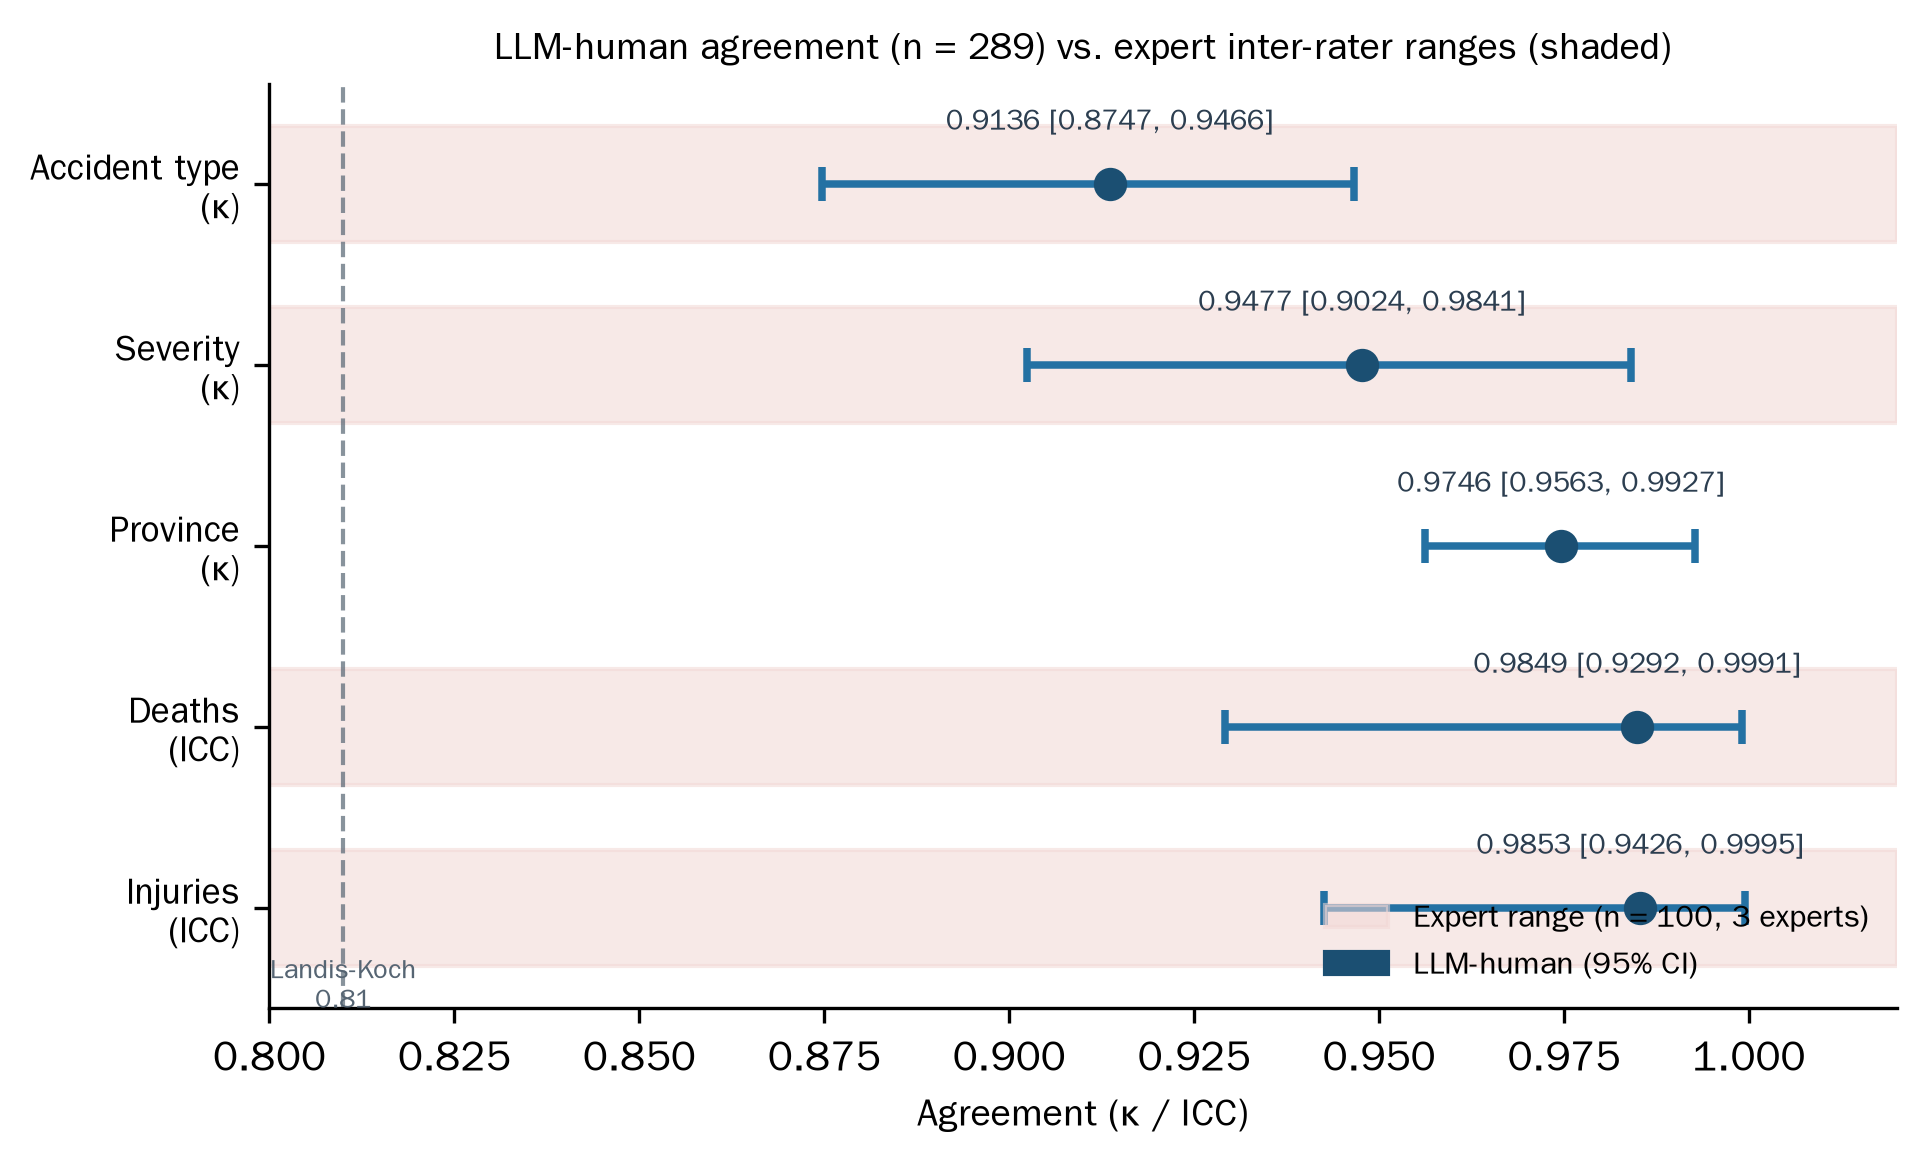
\includegraphics[width=0.85\textwidth]{figures/fig7_kappa.png}
\end{figure}
The sample size was fixed before data collection by the Fleiss' kappa standard-error formula: for expected kappa near 0.90 with a target 95\% confidence-interval half-width of 0.063, the required $n$ is approximately 300, and the observed CIs confirm the design (maximum observed half-width 0.045). The remaining disagreements are concentrated in semantically adjacent accident-type boundaries (e.g., earthwork collapse versus general collapse), where experts disagree with each other at comparable rates, indicating that the residual human-AI divergence reflects genuine task ambiguity rather than systematic LLM error.

\subsection{4.6 Summary of the Evaluation Chain}
The three experiments form a closed argument. Experiment 1 selects the backbone on extraction faithfulness, cost, and speed. Experiment 2 identifies the prompting strategy --- and the two-step judgment design --- that maximizes recall while preserving evidence-bound output. Experiment 3 certifies that the resulting annotations meet expert-level agreement on all six basic features. Together they support the system-level claim of Section 3: the pipeline converts unstructured narratives into a reliable, auditable, causally annotated database.

\section{5. Discussion}
\subsection{5.1 Theoretical implications}
The strategy-ranking reversal between our experiments and Liu et al. [8] is best read as evidence about prompting, not about models. Few-Shot and domain CoT occupy different points in the space of supervision styles: Few-Shot transmits implicit norms through examples, while domain CoT transmits explicit procedure through instructions. Which style wins depends on the model's capability profile --- its in-context pattern-matching efficiency versus its instruction-following alignment --- or on the task's structure; our cross-study contrast cannot separate the two, and Section 4.4.2 states that boundary explicitly. A practical corollary: for the open-model family, Few-Shot is the more reliable default; for instruction-tuned commercial models, domain CoT retains its documented advantage. The Lexical Gatekeeping Effect sharpens this lesson by showing that domain CoT is not merely weaker on some models but actively dangerous when its embedded knowledge is phrased as conditional checks: a poorly designed CoT prompt underperforms a blank prompt (v1 F1 = 0.503 versus Zero-Shot 0.600). Our ablation (Table 7) establishes the causal role of phrasing under controlled conditions --- the phrasing manipulation alone, with the conservative instruction held constant, delivers 0.62 of the total 0.64 recovery on the flagship implicit category. The asymmetry between interrogative and declarative phrasing generalizes a design rule for structured extraction: phrase conditions as clues when recall dominates (safety, screening) and as checks when false positives dominate (legal, financial). This rule holds for any domain where implicit categories predominate and literal evidence is the exception.

\subsection{5.2 Practical implications}
For safety practice, three consequences follow. First, evidence-bound coding makes every causal annotation traceable to a source sentence, converting the database from a statistical object into an auditable one --- safety analysts can verify the grounds of any code without re-reading full reports. Second, the validated agreement levels ($\kappa$ = 0.91--0.97) justify LLM substitution for expert coding of basic fields at industrial scale, at a marginal cost of USD 0.0007 per record (Section 4.3), which places continuous nationwide monitoring within reach of safety regulators. Third, the MECE enumeration procedure offers a template for standardizing any free-text field in safety reporting; its LLM-first orientation --- observe the data, then design the taxonomy --- avoids the unmappable-value failures of rule-first schemes, as evidenced by the 18.9\% $\rightarrow$ 2.9\% reduction of the residual "other" class in the work-task field.

\subsection{5.3 Comparison with prior work}
Table 9 positions CAIEMS against the closest systems. The distinguishing combination is scope: prior systems achieve single-stage extraction [6], single-domain classification [7, 22], or static knowledge artifacts [9, 16], while CAIEMS spans collection to interactive access with formal reliability certification at each stage. The strategy-level comparison with Liu et al. [8] has been treated in Section 4.4; at the system level, the addition of evidence-bound coding and MECE standardization is what makes the database usable for statistical analysis rather than illustrative browsing.

\textbf{Table 9.** Comparison with representative prior systems.}
\begin{table}[htbp]
\centering
\small
\begin{tabular}{cccccccc}
\hline
System & Domain & LLM & Causal taxonomy & Evidence-bound & End-to-end & Agreement validation & Online access \\
\hline
Liu et al. [8] & Aviation & GPT-4o & HFACS & No & No & No & No \\
Kim and Han [7] & Construction (KR) & Claude 3.5 & HFACS & No & No & No & No \\
Ahmadi et al. [6] & Construction (US) & GPT-4.0 & None & No & No & No & No \\
Liu and Luo [9] & Construction & GPT-4o & Accimap & No & Partial & No & No \\
Jiang et al. [16] & Coal mining & LLM & Custom ontology & No & Partial & No & Visualization only \\
CAIEMS (ours) & Construction (CN) & DeepSeek V4 & CAICS (19) & Yes & Yes & Yes ($\kappa$ 0.91--0.97) & Yes (Web + API) \\
\hline
\end{tabular}
\end{table}
\subsection{5.4 Limitations}
Seven limitations bound the current work. (1) The strategy comparison ran on a single model; the model-dependence hypothesis rests on cross-study contrast with Liu et al. [8] rather than a within-study multi-model design. (2) The agreement validation covers six basic features but not the causal codes themselves; expert ground truth for the strategy experiment (three experts, Fleiss' $\kappa$ > 0.85) bounds causal-code reliability indirectly, but a direct $\kappa$ study on causal coding at scale remains future work; correspondingly, the practical substitution claim (Section 5.2) applies to basic fields only. (3) The city-field accuracy (81.5--88.0\%) reflects an administrative-level mismatch (county-level cities reported versus prefecture-level ground truth) that a hierarchical location model could resolve. (4) The multimodal modules are display-oriented: image quality at the source constrains what VLM analysis can contribute, and the 282 VLM descriptions are presented as supplementary material rather than verified annotations. (5) The database covers news-reported accidents, which oversample severe incidents relative to the true accident population; generalization to minor incidents requires regulatory report access. (6) All LLM runs used temperature 0.0 with a single execution per configuration; the reported strategy metrics are point estimates without variance, and low-frequency codes (e.g., C1 with one ground-truth occurrence in the strategy sample) have unreliable per-code estimates. (7) The 972-record silver standard was constructed by pipeline-version agreement with rule-based arbitration rather than independent human re-annotation; its basic-field reliability is bounded by the two source versions, and only the 100-record causal subset carries independent expert validation.

\section{6. Conclusion}
This paper presented CAIEMS, an end-to-end LLM-driven pipeline that converts unstructured Chinese construction accident narratives into a structured, causally annotated, interactive online database. Three results carry the contribution. First, the CAICS five-layer, nineteen-category taxonomy provides a construction-specific causal substrate, with 17,364 evidence-bound codes across 2,623 records. Second, the Lexical Gatekeeping Effect --- identified, diagnosed, and remedied through a two-step judgment design (F1 0.503 $\rightarrow$ 0.656) --- establishes a generalizable prompt-design rule, while the Few-Shot victory over domain CoT (0.669 vs. 0.656) demonstrates that prompting-strategy rankings are model-dependent. Third, the agreement study certifies LLM basic-field annotations at expert inter-rater levels ($\kappa$ = 0.91--0.97, n = 289). Future work extends along three lines: a within-study multi-model test of the model-dependence hypothesis, direct agreement validation for causal coding at scale, and evaluation of the multimodal descriptions once higher-quality accident imagery becomes available.

\section{7. Declarations}
\textbf{Data availability.} The CAIEMS database (2,623 accident records, 17,364 causal codes, CAICS operational definitions, MECE enum definitions) will be released publicly upon publication at a persistent repository. The six prompt templates are reproduced in Appendix A.

\textbf{Code availability.} The extraction pipeline, evaluation scripts, and experiment runners will be released under an open-source license in the same repository as the data upon publication.

\textbf{Ethics declaration.} This study analyzes publicly available news reports and government-published accident briefings. No human subjects, personal data of identifiable individuals, or clinical data are involved.

\textbf{CRediT author statement.} Tianhao Sun (Nanjing Tech University): Conceptualization, Methodology, Software, Data Curation, Formal Analysis, Investigation, Writing --- Original Draft. [Supervisor name] (Nanjing Tech University): Conceptualization, Supervision, Validation, Writing --- Review \& Editing, Funding acquisition.

\textbf{Declaration of competing interest.} The authors declare no competing interests.

\textbf{Funding.} This research received no specific grant from funding agencies in the public, commercial, or not-for-profit sectors.

\textbf{Use of AI tools.} Large language models constitute the research object and the core technical instrument of this study: all extraction, classification, and coding results reported in Sections 3--4 were produced by the evaluated models through the documented pipeline. During manuscript preparation, LLM-based writing assistance was used for language polishing of the English text; all scientific content, experimental design, and data originate from the authors' work and were verified by the authors.

\section*{References}
\begin{enumerate}
\item Kong, F., Ahn, S. (2024). Use of Knowledge Graphs for Construction Safety Management: A Systematic Literature Review. Information, 15(7), 390. https://doi.org/10.3390/info15070390
\end{enumerate}
[2] Togan, V., Mostofi, F., Tokdemir, O.B., Kadioglu, F. (2025). Efficient Management of Safety Documents Using Text-Based Analytics to Extract Safety Attributes From Construction Accident Reports. IEEE Access, 13, 99758-99777. https://doi.org/10.1109/ACCESS.2025.3576442

[3] Devlin, J., Chang, M.-W., Lee, K., Toutanova, K. (2019). BERT: Pre-training of Deep Bidirectional Transformers for Language Understanding. In Proceedings of NAACL-HLT 2019, 4171-4186.

[4] Brown, T., Mann, B., Ryder, N., et al. (2020). Language Models are Few-Shot Learners. Advances in Neural Information Processing Systems, 33, 1877-1901.

[5] OpenAI (2023). GPT-4 Technical Report. arXiv:2303.08774.

[6] Ahmadi, E., Muley, S., Wang, C. (2024). Automatic Construction Accident Report Analysis Using Large Language Models (LLMs). Journal of Intelligent Construction, 3(1). https://doi.org/10.26599/jic.2024.9180039

[7] Kim, D., Han, S. (2024). Systemic Analysis of Fall Accidents Caused by Worker Inattention at Construction Sites: An Integrated Approach using HFACS and LLM. KIBIM Magazine, 14(4), 23-34. https://doi.org/10.13161/kibim.2024.14.4.023

[8] Liu, Q., Li, F., Ng, K.K.H., Han, J., Feng, S. (2025). Accident investigation via LLMs reasoning: HFACS-guided Chain-of-Thoughts enhance general aviation safety. Expert Systems with Applications, 269, 126422. https://doi.org/10.1016/j.eswa.2025.126422

[9] Liu, Q., Luo, X. (2025). Large language model-based knowledge graph construction of unstructured accident reports to improve construction safety. EG-ICE 2025. https://doi.org/10.17868/strath.00093269

[10] Rafindadi, A.D., Shafiq, N., Othman, I., et al. (2023). Data mining of the essential causes of different types of fatal construction accidents. Heliyon, 9(2), e13389. https://doi.org/10.1016/j.heliyon.2023.e13389

[11] Onuchukwu, I.S., Gholizadeh, P., Liko, G., Esmaeili, B. (2024). Nature of Occupational Incidents among Roofing Contractors: A Data Mining Approach. Buildings, 14(3), 595. https://doi.org/10.3390/buildings14030595

[12] Ayhan, B.U., Tokdemir, O.B. (2019). Predicting the outcome of construction incidents. Safety Science, 113, 91-104. https://doi.org/10.1016/j.ssci.2018.11.001

[13] Zhang, L., Hou, Y., Ren, F. (2025). AIR Agent - A GPT-Based Subway Construction Accident Investigation Report Analysis Chatbot. Buildings, 15(4), 527. https://doi.org/10.3390/buildings15040527

[14] Liu, Q., Ding, Y., Luo, X. (2025). Automated knowledge graph-based risk assessment for fall-from-height accidents in construction. Automation in Construction, 179, 106482. https://doi.org/10.1016/j.autcon.2025.106482

[15] Huang, Y., Yan, R., Zhang, Z. (2026). Automated knowledge extraction from marine accident reports using large language models: Graph construction and evaluation. Ocean \& Coastal Management, 272, 108015. https://doi.org/10.1016/j.ocecoaman.2025.108015

[16] Jiang, Y., Nie, B., Wang, J., Peng, P., Wang, L. (2026). Large language model-driven knowledge graph and intelligent analysis for coal mine accidents. Measurement, 277, 121558. https://doi.org/10.1016/j.measurement.2026.121558

[17] Shappell, S.A., Wiegmann, D.A. (2000). The Human Factors Analysis and Classification System-HFACS. Report DOT/FAA/AM-00/7, Office of Aviation Medicine, Federal Aviation Administration.

[18] Wei, J., Wang, X., Schuurmans, D., et al. (2022). Chain-of-Thought Prompting Elicits Reasoning in Large Language Models. Advances in Neural Information Processing Systems, 35, 24824-24837.

[19] Kojima, T., Gu, S.S., Reid, M., Matsuo, Y., Iwasawa, Y. (2022). Large Language Models are Zero-Shot Reasoners. Advances in Neural Information Processing Systems, 35, 22199-22213.

[20] Wang, X., Wei, J., Schuurmans, D., et al. (2023). Self-Consistency Improves Chain of Thought Reasoning in Language Models. In Proceedings of ICLR 2023.

[21] Zhou, D., Schaerli, N., Hou, L., et al. (2023). Least-to-Most Prompting Enables Complex Reasoning in Large Language Models. In Proceedings of ICLR 2023.

[22] Yan, Y., Li, B., Lodewijks, G. (2025). UAV Accident Forensics via HFACS-LLM Reasoning: Low-Altitude Safety Insights. Drones, 9(10), 704. https://doi.org/10.3390/drones9100704

[23] Ahmadi, A., Sharif, S., Banad, Y. (2025). Improving Aviation Safety Analysis: Automated HFACS Classification Using Reinforcement Learning with Group Relative Policy Optimization. arXiv:2508.21201.

[24] Yang, J., Park, S. (2025). LLM-Assisted Knowledge Graph Construction for Managing Road Accident Information From News Articles. IEEE Access, 13, 217846-217865. https://doi.org/10.1109/ACCESS.2025.3648842

[25] Zhang, J., Zhang, W., Wei, Q., Zhong, H., Miao, Y. (2025). GRAG-ProSafe QAS: Graph retrieval-augmented generation for process production safety intelligent question and answer system. Expert Systems with Applications. https://doi.org/10.1016/j.eswa.2025.129947

[26] Shi, D., Gan, S., Zurada, J., Guan, J., Wang, F., Weichbroth, P. (2025). A multi-model approach to construction site safety: Fault trees, Bayesian networks, and ontology reasoning. Expert Systems with Applications, 288, 127817. https://doi.org/10.1016/j.eswa.2025.127817

[27] Xiao, X., Chen, P., Qi, B., et al. (2026). KRAIL: A knowledge-driven framework for human reliability analysis integrating IDHEAS-DATA and large language models. Reliability Engineering \& System Safety, 265, 111585. https://doi.org/10.1016/j.ress.2025.111585

[28] Xuecai, X., Gui, F., Shifei, S., et al. (2024). Accident case data-accident causation model driven safety training method. Process Safety and Environmental Protection, 182, 1208-1226. https://doi.org/10.1016/j.psep.2023.12.042

\appendix
The six prompting strategies are reproduced below in condensed form; the complete prompts are released with the supplementary repository.

\textbf{A.1 S0 Basic Zero-Shot} (system prompt, verbatim core):

\textbf{A.2 S1 Basic Few-Shot}: identical to S0, plus three expert-annotated examples inserted before the user message, each formatted as (accident text $\rightarrow$ JSON output with codes, evidence quotations, and inference notes). Example excerpt: \textit{"{\cjkfont 升降机未经检验合格即投入使用}..."} $\rightarrow$ `{"codes":["M1","M3","M4","F2","T1","H1","H2"], ...}`.

\textbf{A.3 S2 Auto-CoT}: S0 plus the instruction: "First organize your reasoning along the M$\rightarrow$F$\rightarrow$T$\rightarrow$H$\rightarrow$C causal chain step by step, then merge all selected codes into the final JSON `codes` field."

\textbf{A.4 S3 Plan-and-Solve}: S0 plus the instruction: "First draft a brief analysis plan covering the five CAICS layers, then execute the plan and output the final JSON."

\textbf{A.5 S4 CAICS-CoT (ours)}. Two versions were tested. The v1 system prompt phrased every code as a conditional check (excerpt, verbatim):

The v2 system prompt replaced conditional checks with the two-step judgment (excerpt, verbatim):

\textbf{A.6 S5 CAICS-CoT+ (ours)}: five independent API calls, one per layer. Call 1 (M layer): "You are a safety management expert. Identify management-root causes from the accident text. [M1--M5 with cues and inferences] Output JSON: {"M":["M1","M2"],"reasoning":"..."}". Call 2 (F layer) receives "Known management-layer findings: {result\_M}" and so on; each downstream call injects the summaries of all upstream results. A final aggregation call merges the five layer outputs into the unified JSON.

\end{document}